	%%%%%%%%%%%%%%%%%%%%%%%%%%%%%%%%%%%%%%%%%%%%%%%%%%%%%%%%%%%%%%%%%%%%%%%%%%%%%%%%%%%%%%%%%%%%%
	%%									Chapitre 2												%
	%%%%%%%%%%%%%%%%%%%%%%%%%%%%%%%%%%%%%%%%%%%%%%%%%%%%%%%%%%%%%%%%%%%%%%%%%%%%%%%%%%%%%%%%%%%%%
	
	\chapter{Épidémiologie, modélisation et  application aux nématodes des racines}
	\label{chapter2}
	
	\minitoc
	
	%\stcom{Je pense qu'il faudrait enlever ``et des pratiques agronomiques'' au titre de la thèse. Garder tous les logos sur la page de garde ?}
	
	\newpage
	Dans ce chapitre, nous introduisons les bases de notre modèle d'interaction entre plante hôte et nématodes à galles. La première section \ref{sec:epimod} est consacrée à la modélisation en épidémiologie. Dans un premier temps en section~\ref{sec:SIR}, nous décrivons un modèle fondamental en épidémiologie, le modèle compartimental SIR (Susceptible, Infecté, Retiré), qui décrit l’évolution d’une maladie dans une population. Nous  présentons également le nombre de reproduction de base $\mathscr{R}_0$. Dans un deuxième temps, nous présentons  quatre extensions  possibles et non exhaustives du modèle SIR, en lien avec notre stratégie de  modélisation : \ref{sec:latence} la période de latence ; \ref{sec:libres} la forme libre de l'agent pathogène, présente chez la plupart des pathogènes des plantes ; \ref{sec:sais} la saisonnalité, qui joue  un rôle important sur la dynamique des hôtes ; et \ref{sec:resist-virul} l'évolution de la virulence des agents pathogènes lors du déploiement de la résistance génétique des plantes. La deuxième section~\ref{sec:modeles-nematodes} présente les modèles de la littérature consacrés aux nématodes des racines. On retrouve plus particulièrement des modèles décrivant une saison de culture, qui cherchent à déterminer le rendement et la dynamique des nématodes (section~\ref{sec:une-saison}). D'autres modèles se concentrent sur la survie des nématodes pendant l'intersaison (section~\ref{sec:modele-intersaison}). Enfin, quelques modèles considèrent plusieurs saisons de culture, mais peu de modèles mécanistes type SIR (section~\ref{sec:plusieurs-saisons}).  Pour finir, à partir de tous ces éléments, nous présentons en section~\ref{sec:notre-strategie} notre stratégie de modélisation, pour décrire la dynamique saisonnière d'interaction entre une succession de plantes hôtes susceptibles ou résistances et les nématodes à galles.
	
	
\section{Épidémiologie végétale et modélisation}
\label{sec:epimod}
	
	L'épidémiologie est définie comme l'étude de la propagation de maladies dans l'espace et le temps. Plus particulièrement, l'épidémiologie végétale est définie comme \og l’étude des populations d'agents pathogènes dans les populations de plantes hôtes, et les maladies qui en résultent sous l'influence de l'environnement et des interférences humaines \fg{} \citep{Kranz1990}. 
	Au milieu du XX\fup{ème} siècle l’épidémiologie végétale  opéra une transition importante en passant d'une discipline qualitative  vers une discipline plus quantitative \citep{Madden2007}. \citet{Large1952} a montré l’intérêt des courbes de progression de maladies pour prédire les pertes de rendement. Par la suite, \citet{Vanderplank1960} eut l'idée radicale  qu’une analyse basée sur des modèles était essentielle pour comprendre les processus de progression d’une maladie et pour établir des stratégies de contrôle.  De bien des manières, le premier livre de \citet{Vanderplank1963} a  contribué à la naissance de la théorie de l’épidémiologie végétale basée sur des processus en dynamique des populations et sur des données empiriques.
	
	
	
	Les modèles en compartiments sont une des bases de l'épidémiologie mathématique \citep{Anderson1991, Dieckmann2000}. Ils consistent à diviser la population hôte en autant de compartiments que d’états cliniques et à relier ces compartiments entre eux par des flux d’individus. En 1766, Daniel Bernoulli inventa le tout premier modèle compartimental   permettant d'estimer l’efficacité de l'inoculation à faible dose de la variole comme  mesure préventive.
	De nombreux autres scientifiques, ont apporté leurs contributions dans le domaine de l'épidémiologie mathématique. 
\citet{Hamer1906} a dans les premiers exprimé le nombre de nouveaux cas pendant un intervalle de temps en fonction du nombre individus susceptibles et infectés. Il faut cependant attendre les travaux de \citet{Ross1911} et \citet{McKendrick1912} sur le paludisme pour que la loi d'action de masse rencontrée en chimie soit appliquée à des modèles épidémiologiques \citep{Heesterbeek2005}. Ce principe fondateur de l'épidémiologie mathématique stipule que le taux de contact entre individus susceptibles et infectés (et par conséquent le nombre de nouveaux cas) est proportionnel aux densités de ces deux sous-populations. Fondé sur ce principe, \citet{Kermack1927} publient par la suite un modèle fondamental en épidémiologie, le modèle SIR, que nous présentons ci-dessous.
	
	
	
\subsection{Un modèle simple en épidémiologie : SIR}
\label{sec:SIR}
	
	Le modèle SIR a pour  but  de décrire la dynamique de transmission d’une maladie dans une population structurée en individus sains  (\og Susceptible \fg{} $S$), infectés (\og Infected\fg{} $I$) et retirés (\og Removed \fg{} $R$). Le compartiment R contient des individus qui ne participent plus à l'infection, qui sont guéris et immunisés. 
Les compartiments peuvent correspondre à  un nombre d'individus ou à une densité de population, c'est-à-dire une proportion d'individus dans une population donnée ou un nombre d'individus par unité de surface. 
Le modèle SIR est généralement formulé en termes d'équations différentielles ordinaires, formalisme que nous retenons ci-après.
	
\subsubsection{Un modèle SIR avec démographie}
	
	Nous représentons une version du modèle SIR avec  démographie, fondé sur  le modèle historique de \citet{Kermack1932} et représenté sur la \autoref{fig:SIR}.
	
	\begin{figure}[ht]
	  \centering
	  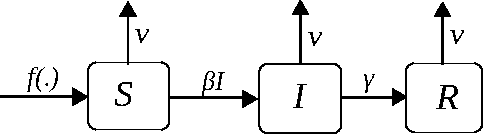
\includegraphics[width=0.6\linewidth]{SIR.pdf}
	  \caption[Diagramme du modèle SIR]{Diagramme du modèle SIR. Les compartiments représentent les individus sains ($S 
	  $), infectés ($I$) et retirés ($R$). $\beta I$ correspond à la force d'infection qui fait passer de $S$ à $I$ et 
	  $f(.)$ le flux des naissances entrant en $S$. Le paramètre $\beta$ désigne le taux de transmission, $\gamma$ le 
	  taux de guérison et $\nu$ le taux de mortalité naturelle.}
	  \label{fig:SIR}
	\end{figure}
	
Nous pouvons écrire ce modèle sous forme d'un système d'équations différentielles ordinaires :
	\begin{equation}
	  \left\{
	    \begin{aligned}
	      \frac{dS}{dt} &= f(.) - \beta SI- \nu S,\\
	      \frac{dI}{dt} &= \beta SI - \gamma I - \nu  I, \\         
	      \frac{dR}{dt} &= \gamma I - \nu R.  
	    \end{aligned}
	  \right.
	  \label{eq:SIR}
	\end{equation}
	
	Les variables d'état $S$, $I$ et $R$ dépendent du temps $t$. 
Connaissant les conditions initiales $S(0), I(0), R(0)$ à $t=0$, on peut déduire de ces équations l'évolution du système au cours du temps.
	
	Les hypothèses du modèle sont les  suivantes, en ce qui concerne les \textbf{paramètres démographiques} : 
\begin{enumerate}[label=\roman*.]
\item  $f(.)$ est une fonction qui représente les naissances par unité de temps. $f$ est positive et c'est généralement une fonction croissante de la population totale $N=S+I+R$. On suppose dans ce modèle que les individus naissent sains, donc $f$ est une entrée du compartiment $S$.
\item $\nu$ est le taux  de mortalité \og naturelle \fg{}, \textit{i.e.} indépendant de la maladie.
\end{enumerate}
et en ce qui concerne les \textbf{paramètres épidémiologiques} :
\begin{enumerate}[label=\roman*.,resume]
\item On suppose que la population est répartie de manière homogène et que la transmission est densité-dépendante, \textit{i.e.} qu'elle suit la loi d’action de masse $\beta S I$, où $\beta$ est le taux de transmission de la maladie. $\beta I$ représente la force d'infection ; d'autres formes sont présentées dans l'encadré~\ref{infection}, page~\pageref{infection}.
\item On suppose que les individus infectés sont immédiatement infectieux.
\item Les individus infectés guérissent et sont immunisés à un taux $\gamma$. 
\item Il n'y pas de surmortalité (ou agressivité) due à la maladie. Pour l'introduire, il faudrait un ajouter un  terme $- \alpha I$ à la deuxième équation du système~\eqref{eq:SIR} (qui représente l'évolution des individus $I$),
 avec $\alpha$  le taux de mortalité due à la maladie.
\end{enumerate}
	
	
	Le modèle SIR présenté en~\eqref{eq:SIR} peut se décliner de plusieurs manières. On peut par exemple considérer un modèle \textbf{en population constante}, où les naissances compensent les morts ($f=\nu N$) :
	\begin{equation}
	   \left\{
	     \begin{aligned}
	       \frac{dS}{dt} &= \nu (N - S) - \beta SI,\\
	       \frac{dI}{dt} &= \beta SI - (\gamma +\nu) I, \\         
	       \frac{dR}{dt} &= \gamma I- \nu R, 
	     \end{aligned}
	   \right.
	   \label{eq:SIR-Ncst}
	\end{equation}
	
	ou encore un modèle \textbf{sans démographie}, dans lequel il n'y a ni naissances ($f=0$) ni morts ($v=0$) : 
	\begin{equation}
		\left\{
		\begin{aligned}
			\frac{dS}{dt} &=-\beta SI,\\
			\frac{dI}{dt} &= \beta SI - \gamma I, \\         
			\frac{dR}{dt} &= \gamma I.
		\end{aligned}
		\right.
		\label{eq:SIR-nodemo}
	\end{equation}
	
	De nombreuses autres variantes du modèle SIR existent.  Par exemple, le modèle SIS permet de décrire une maladie sans immunité suite à une infection, dans lequel les individus rétablis sont susceptibles d'être réinfectés.  La possibilité intermédiaire d'une immunité temporaire peut être décrite par un modèle de type SIRS, dans lequel les individus guéris $R$ redeviennent susceptibles $S$ au bout d'un certain temps, suite à la perte de leur immunité \citep{Brauer2012}.
	
\begin{encadre2}{Force d'infection}
\label{infection}
La force d'infection $g(I,N)$ est le taux auquel un individu susceptible $S$ devient infecté. En supposant que les individus des différents compartiments sont répartis de manière homogène dans la population, on  peut décomposer la force d'infection comme suit :
	  \begin{equation*}
	    g(I,N) = c(N) \: \frac{I}{N} \: e,
	  \end{equation*}
où $c(N)$ représente le nombre de contacts par unité de temps et par individu, $\frac{I}{N}$ la probabilité que le contact ait lieu avec un individu $I$ et $e$ l'efficacité ou l'infectiosité d'un contact avec un individu $I$ (supposée constante). $c(N)$ prend généralement deux formes distinctes :
	  \begin{itemize}
\item Soit $c(N)= c_0 N$, \textit{i.e.} le taux de contact est proportionnel à la taille ou la densité de la population. On parle alors de \textbf{transmission densité-dépendante} ou de loi d'action de masse :
	    \begin{equation*}
	      g(I,N) = g(I) = c_0 e I.
	    \end{equation*}
C'est le cas du modèle SIR présenté en~\eqref{eq:SIR}, avec $\beta=c_0 e$ comme taux de transmission.
\item Soit $c(N)= c_1$, \textit{i.e.} le taux de contact est constant. On parle alors de \textbf{transmission fréquence-dépendante} :
	    \begin{equation*}
	      g(I,N) = c_1 e \frac{I}{N}.
	    \end{equation*}
 Le taux de transmission $\beta'=c_1 e$ n'est pas le même que le taux $\beta$ du cas précédent (grandeurs et unités différentes). 
 \end{itemize}
{\small \textsc{Remarque --} Dans le cas où la taille ou la densité $N$ de la population est constante, comme par exemple dans les deux variantes du modèle SIR \eqref{eq:SIR-Ncst} et \eqref{eq:SIR-nodemo}, les transmissions densité-dépendante et fréquence-dépendante sont équivalentes, avec $\beta=\beta'/N$.}
\par\medskip
	  La transmission densité-dépendante est très largement employée dans les modèles épidémiologiques, l'hypothèse que le taux de contact augmente linéairement avec la densité de population étant assez réaliste. Cependant, quand la densité de population devient très élevée, cette hypothèse est moins fondée. La transmission fréquence-dépendante est elle généralement choisie pour les maladies sexuellement transmissibles, le nombre de partenaires étant supposé indépendant de la taille ou densité de population.  Outre ces deux formes classiques pour la force d'infection, il existe d'autres modèles de transmission, qui sont par exemple présentés dans \citet{McCallum2001}.  
	\end{encadre2}
	
	
\subsubsection{Équilibres et taux de reproduction de base}
\label{sec:R0}
	Les équilibres du système (\ref{eq:SIR}) dépendent de la forme de la fonction de naissance~$f$. Le premier équilibre est $\mathcal{E}^*=(S^*,0,0)$, où $S^*$ vérifie $f(\mathcal{E}^*) = \nu S^*$.
\begin{itemize}
\item Si cette équation n'est vérifiée que pour $S^*=0$, par exemple quand $f$ est une fonction linéaire de la (densité) de population totale $f=kN$ (avec $k\neq\nu$), le premier équilibre est l'\textbf{équilibre trivial} $(0,0,0)$.
\item Si cette équation est vérifiée pour $S^*>0$, par exemple quand $f$ est une fonction constante $f=k$, alors cet équilibre $(S^*,0,0)$ est appelé \textbf{équilibre sans maladie} (\og disease free equilibrium \fg{} ou DFE en anglais), car il caractérise une situation où la maladie est absente de la population.
\end{itemize}
	
	Le second équilibre  $\bar{\mathcal{E}}=(\bar{S},\bar{I},\bar{R})$ est  appelé \textbf{équilibre  endémique}. Cet équilibre correspond à une situation où la maladie persiste dans la population et est donné par le système suivant :  
	\begin{equation}
	\left\{
		\begin{aligned}
		\bar{S} &= \frac{\nu+\gamma}{\beta}, \\
		\bar{I} &= \frac{f(\bar{S},\bar{I})}{\nu+\gamma}-\frac{\nu}{\beta},  \\
		\bar{R} &= \frac{\gamma\bar{I}}{\nu}. \\
		\end{aligned}
		\right.
	\label{sys1}
	\end{equation}
Cet équilibre n'existe que si $\bar{I}>0$, ce qui dépend de la fonction $f$ et des valeurs des paramètres.
	
	On suppose qu'il existe bien un équilibre sans maladie $\mathcal{E}^*=(S^*,0,0)$ tel que $S^*=\frac{f(\mathcal{E}^*)}{\nu}>0$. On peut alors définir le \textbf{taux de reproduction de base} du modèle SIR~\eqref{eq:SIR} comme suit :
	\begin{equation}
	  \mathscr{R}_0=\frac{\beta S^*}{v+\gamma}.
	  \label{R0}
	\end{equation}
	
	Le taux de reproduction de base est un concept clé en épidémiologie. Dans une population composée d’individus sains ($N=S^*$) dans laquelle on introduit un individu infecté, $\mathscr{R}_0$ correspond au nombre de cas secondaires d'infection engendrés par cet individu ($\beta S^*$) au cours de sa période infectieuse ($\frac{1}{\gamma + v}$) \citep{Dieckmann2000,vandenDriessche2002}. Si  $\mathscr{R}_0<1$ la maladie ne peut pas se propager, si $\mathscr{R}_0>1$ il peut y avoir une épidémie.
	
	Au niveau mathématique, $\mathscr{R}_0$ est lié à la stabilité locale de l'équilibre sans maladie : si $\mathscr{R}_0<1$ l'équilibre est asymptotiquement stable, si $\mathscr{R}_0>1$ il est instable.
En général ce seuil est lié à l'existence de l'équilibre endémique. Dans le cas, par exemple, du modèle SIR~\eqref{eq:SIR} avec naissances constantes $f=k$ :
\begin{itemize}
	\item si $\mathscr{R}_0<1$, on a un unique équilibre stable sans
	  maladie et la maladie ne peut pas s'installer ; 
	\item si $\mathscr{R}_0>1$ l'équilibre sans maladie est instable, l'équilibre endémique existe et il peut y avoir persistance de la maladie.
	\end{itemize}
	
\begin{encadre2}{Le taux de reproduction de base $\mathscr{R}_0$}
\label{encadre:R0}
 À l’origine,  $\mathscr{R}_0$ provient de la démographie \citep{Heesterbeek2002}. C’est en 1886 qu’il est introduit pour la première fois par Richard Böckh  alors qu’il cherchait à exprimer le nombre moyen de filles qu’une femme va engendrer au cours de sa vie \citep{Bockh1886}.
 \citet{Dublin1925}  définissent le $\mathscr{R}_0$ ainsi :
	  \begin{equation*}
	    \mathscr{R}_0= \int_{0}^{\infty} F(a)\beta(a) da,
	  \end{equation*}
 avec $F(a)$ la probabilité pour une femme de survivre à l’âge $a$ et $\beta(a)$ le taux de naissance de filles.
\par
Si la notion de densité seuil est apparue relativement tôt en épidémiologie, dans les travaux de \citet{Ross1911} sur le paludisme et de \citet{Kermack1927} pour les maladies à transmission directe, elle n’était au départ pas liée au $\mathscr{R}_0$. Le concept du taux de reproduction de base n’est introduit que bien plus tard  par \citet{Macdonald1952} lors de ses recherches sur le paludisme.
\par
Le concept est ensuite repris indépendamment par \citet{Dietz1975}  et \citet{Hethcote1975} pour les maladies à transmission directe. Enfin, il prend son essor dans les années 1990 grâce aux travaux méthodologiques de \citet{Diekmann1990} et au livre de référence en épidémiologie de \citet{Anderson1991}, qui lui accordent une large part.
\end{encadre2}
	
	
\subsection{Extensions du modèle SIR}
\label{sec:ext}
	 
	Le  succès du modèle SIR introduit par \citet{Kermack1932} est qu'il peut prédire le comportement de nombreuses maladies \citep{Brauer2012}. D'ailleurs, bien que les modèles compartimentaux aient été développés tout d'abord pour la compréhension et le contrôle  des épidémies  humaines puis animales, ils sont  de plus en plus appliqués en épidémiologie végétale \citep{Vanderplank1963, Madden2007,Gilligan2008}. %Van der Plank, est l'un des pionniers dans l'élaboration d'un cadre de modélisation pour l'étude de maladies transmissibles aux  végétaux (VanderPlank1960, VanderPlank1963). 
	En épidémiologie végétale les plantes sont pratiquement immobiles, mais la propagation des maladies est possible grâce à la dissémination des agents pathogènes par le vent, par l’eau ou par un vecteur \citep{Madden2007}. De nombreux modèles en épidémiologie végétale sont basés sur le modèle SIR présenté ci-dessus en section~\ref{sec:SIR}. Dans ce cadre, les variables d'état ($S,I,R$) désignent un nombre, une biomasse ou une densité de plantes, de racines, de fruits, \textit{etc.} Nous allons à présent décrire quatre extensions  possibles du modèle SIR, qui sont pertinentes en épidémiologie végétale et plus particulièrement avec notre approche de modélisation.
	
	%Les premières publications concernant les concepts associés aux modèles appliqués aux pathogènes télluriques sont dans les articles pionniers de Dimond \& Horsfall (37) et Baker (3). Par la suite, 
	%des  auteurs comme Gilligan  ont apporté une grande contribution dans le domaine de la modélisation des pathogènes télluriques \citep{Gilligan1983, Gilligan1985 Gilligan1990, Gilligan1995, Gilligan1994, Perry1983}. Toutefois, contrairement  à la  modélisation abondante des pathogènes transmis par voie aérienne \citep{Waggoner1977, thrall2002, Brown2002, Mundt2002}, la modélisation des pathogènes transmis par le sol est encore trop rare dans le  domaine de l'épidémiologie végétale \citep{Gilligan
	%1995, Thrall2007, Otten2003}.
	
\begin{quote}
	  \textsc{Notations} -- En épidémiologie humaine ou animale, le compartiment $S$ des modèle SIR désigne des individus sensibles (\og Susceptible \fg{} en anglais). En santé des plantes, le terme sensible est souvent utilisé pour désigner un trait génétique de la plante (voir~\ref{terminologie} page~\pageref{terminologie}). C'est pourquoi nous utilisons ci-dessous la notation $H$ pour les plantes saines (\og Healthy \fg{} en anglais). Par souci de cohérence avec notre modèle présenté en section~\ref{sec:notre-strategie}, nous conservons la notation classique $E$ pour les hôtes infectés en période de latence, introduite en section~\ref{sec:latence}, mais nous utilisons la notation $P$ pour la forme libre du pathogène, introduite en section~\ref{sec:libres}.
	\end{quote}

\subsubsection{La période de latence}
\label{sec:latence}
	
	Quand un individu est attaqué par un agent pathogène, il y a une période de latence durant laquelle l’agent pathogène se développe, mais l’individu hôte n’est pas encore infectieux \citep{Madden2007}. Il peut être pertinent de l'inclure dans un modèle épidémiologique, car cette période  est parfois  plus longue que la période d'infectiosité  \citep{Vanderplank1963}. Ainsi, le modèle SIR de la section précédente~\ref{sec:SIR} peut être étendu pour inclure la période de latence \citep[par exemple]{Dieckmann2000}. En épidémiologie humaine ou animale, on parle d'individus exposés (\og Exposed \fg{} en anglais) à l'infection, d'où la notation  $E$ pour le stade latent, que nous reprenons ici.
	
	À titre d'exemple, nous présentons un modèle HEIR sans démographie, où la population est mesurée en densité de racines (\autoref{fig:HEIR}). 
	
	\begin{figure}[ht]
	  \centering
		  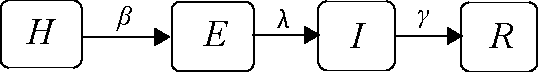
\includegraphics[width=0.6\linewidth]{HEIR}
		  \caption[Diagramme du modèle du modèle HEIR sans démographie]{Diagramme du du modèle HEIR sans démographie.  
		  Les compartiments  représentent les densités  de  racines saines ($H$), latentes  ($E$), infectées ($I$) et 
		  retirées  ($R$).
		  Le paramètre $\beta$ désigne le taux de transmission, $1/\lambda$  la durée de la période de latence et $1/
		  \gamma$ la durée de la période infectieuse.}
		  \label{fig:HEIR}
	\end{figure}
	
	En s'appuyant sur le modèle~\eqref{eq:SIR-nodemo}, nous pouvons donc écrire ce modèle HEIR selon le système d'équations différentielles suivant :
	\begin{equation}
	  \left\{
	    \begin{aligned}
	      \frac{dH}{dt} &= -\beta H I,\\
	      \frac{dE}{dt} &= \beta H I  - \lambda E, \\         
	      \frac{dI}{dt} &= \lambda E -  \gamma  I, \\
	      \frac{dR}{dt} &= \gamma I.  
	    \end{aligned}
	  \right.
	  \label{eq:HEIR}
	\end{equation}
	La différence avec le modèle~\eqref{eq:SIR-nodemo} est qu'après l'infection (flux $\beta H I$), l'agent pathogène se développe  pendant un temps $1/\lambda$ dans les racines infectées de manière latente $E$, avant que ces racines ne deviennent infectieuses $I$.
	
	

\subsubsection{La forme libre de l'agent pathogène}  
\label{sec:libres}
	
	De nombreux parasites telluriques ou aériens des plantes (bactéries, champignons, virus ou nématodes) présentent un cycle biologique complexe, où la transmission se fait via un stade de développement en dehors de la plante hôte \citep{Dwyer1994, Godfray1997}. En effet, les parasites doivent faire face à l’immobilité des plantes et donc développer des stratégies pour transmettre l’infection. Cela peut se faire par la production et dispersion massive de spores chez les champignons \citep{Agrios2005}, via un insecte vecteur pour les virus \citep{Madden2000}, ou encore grâce à une forme libre dans le sol pour les nématodes racinaires \citep{Nilusmas2017}.
Les formes libres sont souvent des formes de survie permettant au parasite non seulement de se disperser, mais aussi de survivre en l'absence d'hôtes. Chez les nématodes à kystes, les œufs peuvent rester dans le sol sous forme de kystes pendant des mois, la libération des larves dans le sol n'intervenant qu'en présence de certains exsudats de la plante \citep{Perry2018}.
	
	
	Nous présentons à titre d'exemple le modèle proposé par \citet{Cunniffe2011}, qui décrit la dynamique d'infection d'une plante par un champignon tellurique, avec un inoculum primaire sous forme libre dans le sol. Cet inoculum ($P$) correspond à des spores, des sclérotes ou encore des débris de racines précédemment colonisées. Les racines sont scindées en racines saines ($H$) et infectées ($I$). Le modèle intègre la dynamique de l'inoculum, la croissance de l'hôte et les processus d'infection des racines. Il correspond au système suivant :
	\begin{equation}
	  \left\{
	    \begin{aligned}
	      \frac{dP}{dt} &= \nu I -  \gamma P, \\
	      \frac{dH}{dt} &= \eta  \big(\kappa - (H + I)  \big) -  \big(\beta_p P + \beta_s I  \big)H,\\
	      \frac{dI}{dt} &= \big(\beta_p P +  \beta_s I  \big) H - \mu I.\\
	    \end{aligned}
	  \right.
	  \label{eq:PHI}
	\end{equation}
	L'inoculum dans le sol perd son infectiosité à un taux $\gamma$ et est reconstitué par les racines infectées à un taux $\nu$. La croissance du tissu racinaire est \og affine \fg{}, avec un taux constant $\eta\kappa$ pour les petites densités de racines (saines et infectées), qui diminue quand les racines s'approchent de leur capacité de charge $\kappa$. Il y a deux sources d'infection pour les racines saines $S$ : l'inoculum $P$ qui génère les infections primaires associées au taux de transmission $\beta_p$ ; et les racines infectées $I$, qui génèrent les infections secondaires associées au taux de transmission $\beta_s$. Dans les deux cas la transmission est supposée densité-dépendante, tout comme dans le modèle SIR~\eqref{eq:SIR} présenté en début de chapitre. Enfin, le champignon induit une mortalité des racines infectées à un taux constant $\mu$. 
	Dans ce même article, le modèle~\eqref{eq:PHI} est étendu pour prendre en compte un pathogène antagoniste aux champignons telluriques, utilisé comme agent de lutte biologique.
	
	L'existence d'une forme libre est particulièrement importante pour les agents pathogènes des agro-écosystèmes saisonniers, comme cela est décrit dans la section suivante.
	
	
\subsubsection{La saisonnalité}
\label{sec:sais}
	
	Les agro-écosystèmes saisonniers sont marqués par l'absence périodique de l'hôte, due à la récolte. 
Cette période d'absence exerce de forts goulots d’étranglement démographiques sur les populations d'agents pathogènes. Pour survivre, les agents pathogènes se tournent vers des hôtes alternatifs ou développent des stades sous forme libre (voir section~\ref{sec:libres} ci-dessus) leur permettant de supporter de longues périodes sans hôte. 
	
	Dans un système saisonnier, l'infection est initiée par un inoculum primaire, provenant d'une forme libre du pathogène, de pathogènes hébergés par des plantes sauvages ou de débris de plantes de la saison précédente. Cette infection primaire est suivie d'infections secondaires, \textit{i.e.} des infections de plante à plante \citep{Campbell1990}. Lorsque plusieurs cycles d’infections secondaires se succèdent au cours d’une saison, on parle de maladie polycyclique. À l'inverse, si la maladie repose principalement sur les infections primaires et qu'il n’y a qu’un seul cycle d’infection à partir d'une forme libre de survie, la maladie est dite monocyclique.
À la fin de la saison de culture, l'agent pathogène adopte une stratégie de survie pour affronter l’absence de l’hôte jusqu'à la saison suivante. 
	 
	La saisonnalité est modélisée par des forçages périodiques continus \citep{Murray2013} ou via des modèles semi-discrets, qui permettent d'introduire des événements discrets dans une dynamique continue. Ces modèles sont particulièrement adaptés aux agro-écosystèmes saisonniers : la partie continue représente la dynamique des interactions plante-pathogène pendant la saison de culture ; la partie discrète correspond à l'intersaison et aux changements abrupts qui affectent les populations au moment de la récolte et de la plantation. Le formalisme semi-discret est illustré sur la \autoref{fig:semi-discret}
	
	 \begin{figure}[ht]
	  \centering
		  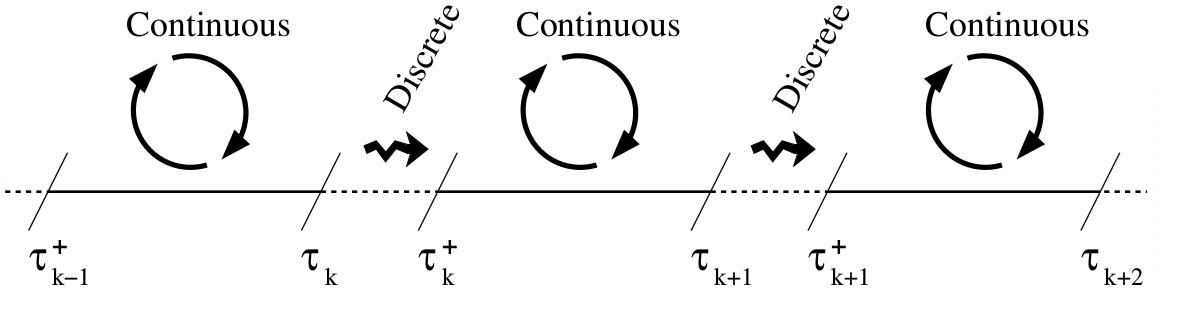
\includegraphics[width=.9\linewidth]{semi-discrete.png}
		  \caption[Illustration du formalisme semi-discret.]{Illustration du formalisme  semi-discret.
		    Le trait plein de l’axe du temps représente les phénomènes continus pour $t \in (\tau_k;\tau_{k+1})$  
		    (\textit{e.g.} cycles d’infection, croissance de l'hôte). Le trait discontinu représente les phénomènes 
		    discrets pour $t = \tau_k$ ($e.g$  récolte et plantation de l'hôte, survie du parasite sous forme libre).
		    D'après \citet{Mailleret2009}.}
		  \label{fig:semi-discret}
	 \end{figure}
	
	\citet{Shaw1994} est le premier à avoir utilisé un modèle semi-discret pour décrire la dynamique d'une épidémie végétale. Il a montré qu'un tel modèle peut conduire à des dynamiques chaotiques, tandis que sans discontinuités, les modèles convergent vers des équilibres stables. Par la suite, des modèles semi-discrets ont été utilisés dans des agro-écosystèmes saisonniers pour étudier la persistance d'agents pathogènes \citep{Madden2002}, l'évolution et la coexistence de pathogènes \citep{Vandenberg2010,Vandenberg2011,Hamelin2011,Mailleret2012}, ou encore pour déterminer des stratégies de déploiement de plantes résistantes \citep{Fabre2012,Fabre2015}. Nous en présentons deux ci-dessous : le modèle de  \citet{Vandenberg2011} et celui de \citet{Mailleret2012}.
	
	%\citet{Madden2002} : modèle  type SEIR avec saisonnalité ; conditions nécessaires à la persistance à long terme d'une maladie végétale après l'introduction d'un micro-organisme pathogène dans une culture annuelle sensible .
	
	
	Le modèle de \citet{Vandenberg2011} est fondé sur un modèle épidémiologique classique décrivant l'évolution des densités d'hôtes sains ($H$) ou infectés ($I$) pendant la saison de culture, auquel on introduit une forme libre de survie du pathogène ($P$) présente uniquement pendant l'intersaison. Il intègre également la croissance de la plante hôte. La dynamique du modèle est décrite ci-dessous et illustrée dans la \autoref{fig:vandenberg}.
	
	\begin{figure}[ht]
	  \centering
	  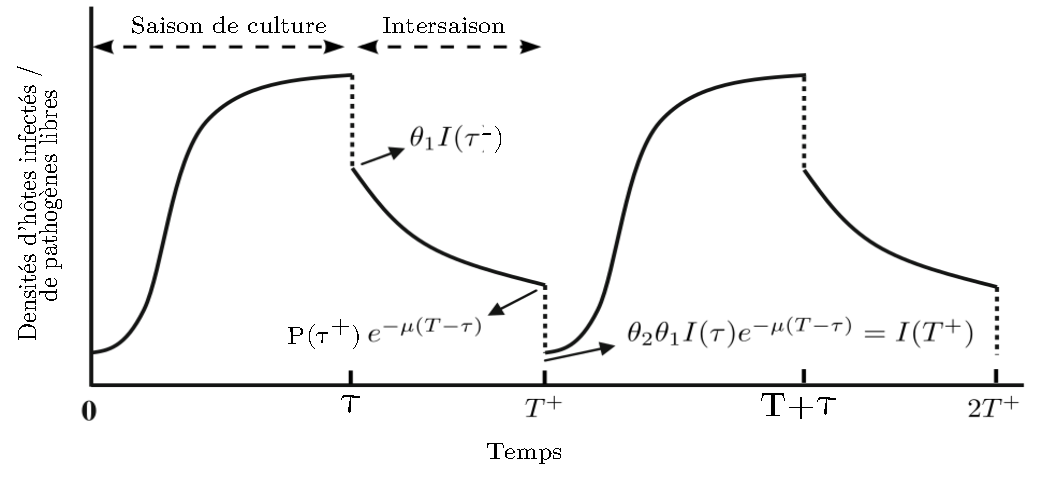
\includegraphics[width=1\linewidth]{vandenberg_sais.pdf}
	  \caption[Dynamique du modèle épidémiologique semi-discret de \citet{Vandenberg2011}]{Dynamique du modèle 
	  épidémiologique semi-discret de \citet{Vandenberg2011}, décrit dans les équations (\ref{eq:vandenberg-saison}-
	  \ref{eq:vandenberg-plant}). L'évolution de l'épidémie est représentée en suivant : la densité d'hôtes infectés 
	  ($I$) pendant les saisons de cultures, \textit{i.e.} pour $t\in(nT^+,nT+\tau^-)$, avec $n=0,1$ ; et la densité de 
	  pathogènes sous forme libre ($P$) pendant l'intersaison, \textit{i.e.} pour $t\in(nT+\tau^+,(n+1)T^-)$. Les sauts 
	  représentent les récoltes ($nT+\tau$) ou les plantations ($nT$) avec $P(\tau^+)=\theta_1 I(\tau^-)$, 
	  $P(T^-)=P(\tau^+)e^{_\mu(T-\tau)}$, $I(T^+)=\theta_2P(T^-)$. 
	   Adapté de \citet{Vandenberg2011}.}
	  \label{fig:vandenberg}
	\end{figure}
	
	On considère la saison $n$, avec $n=0,1,\ldots$
\begin{enumerate}
\item \emph{Saison de culture, soit $t\in(nT^+,nT+\tau^-)$}\quad
Le pathogène sous forme libre est absent, la croissance, la mortalité et l'infection de la plante hôte sont représentées : 
	\begin{equation}
	  \left\{
	    \begin{aligned}
	      P~ &= 0, \\
	      \frac{dH}{dt} &=  f(H,I) - \beta HI - \nu H,   \\
	      \frac{dI}{dt} &= \beta HI - (\nu+\alpha) I,
	    \end{aligned}
	  \right.
	  \label{eq:vandenberg-saison}
	\end{equation}
	avec $f(H,I)$ la fonction de croissance des hôtes, $\beta$ le taux de transmission supposée densité-dépendante, $\nu$ le taux de mortalité naturelle des hôtes et $\alpha$ l'agressivité, \textit{i.e} la mortalité induite par le pathogène.
	\item  \emph{Récolte, soit $t=nT+\tau$}\quad
	  À la fin de chaque saison de culture, les plantes sont arrachées et le pathogène se tourne vers une stratégie de survie ($P$):
	  \begin{equation}
	    \left\{
	      \begin{aligned}
	        P(nT+ \tau^{+}) &= \theta_1 I(nT+\tau^{-}),\\
	        H(nT+ \tau^{+}) &=0,   \\
	        I(nT+ \tau^{+}) &=0,
	      \end{aligned}
	    \right.
	    \label{eq:vandenberg-recolte}
	  \end{equation}
	  avec $\theta_1\in(0,1)$ la proportion d'hôtes infectés ($I$) qui alimentent la forme libre du pathogène ($P$). 
	\item  \emph{Intersaison, soit $t\in(nT+\tau^+,(n+1)T^-)$}\quad
	  L'hôte est absent et le pathogène sous forme libre  meurt à un taux $\mu$ :
	  \begin{equation}
	    \left\{
	      \begin{aligned}
	        \frac{dP}{dt} & = -\mu P, \\
	        H &= 0, \\
	        I~ &= 0. \\
	        \end{aligned}
	    \right.
	    \label{eq:vandenberg-intersaison}
	\end{equation} 
	\item  \emph{Nouvelle saison, soit $t=(n+1)T$}\quad
	  Au début de la saison de culture suivante, une proportion $\theta_2 \in (0,1)$ des pathogènes sous forme libre retournent dans l'hôte et initient la phase épidémique :
	  \begin{equation}
	   \left\{
	      \begin{aligned}
	        P((n+1)T^{+}) &= 0,\\
	        H((n+1)T^{+}) &=H_0 - I((n+1)T^{+}),   \\
	        I((n+1)T^{+}) &=\theta_2 P((n + 1)T^-),
	      \end{aligned}
	    \right.
	    \label{eq:vandenberg-plant}
	  \end{equation}
	  où  $H_0$ est la densité de culture au début de chaque saison, supposée constante.
	\end{enumerate}	
	
	Les auteurs ont étudié l'influence de deux compromis : l’un entre transmission ($\beta$) et agressivité ($\alpha$) et l'autre entre transmission et survie du pathogène sous forme libre ($\mu$). Notamment, ils ont montré  que des durées d'intersaison plus longues sélectionnent des taux de transmission $\beta$ plus élevés dans le cas du compromis $\beta$--$\alpha$, mais plus faibles dans le cas du compromis $\beta$--$\mu$. En l’occurrence ils ont démontré que dans ce système, l’évolution tend a maximiser le $\mathscr{R}_0$ du pathogène.
Dans un environnement périodique,  $\mathscr{R}_0$ est obtenu en linéarisant le système au voisinage de l'état stationnaire sans maladie \citep{Bacaer2006, Bacaer2007}.

	%\citet{Vandenberg2010} par différents  modèles en temps continu
	%avec des dynamiques d’infections dite aérienne ou tellurique combiné avec des épisodes discrets, ont étudié dans quelle mesure l'absence périodique d'hôte  engendre un branchement évolutif. En se basant sur des simulations numériques, 
	%les auteurs ont conclu que \og la périodicité de la disponibilité des hôtes
	%ne permet pas de générer un branchement évolutif, comme observée chez de nombreux agents pathogènes des plantes \fg{}.  
	
	Le second modèle présenté est celui de \citet{Mailleret2012}, basé sur le modèle de \citet{Madden2002}. Il décrit la dynamique épidémique saisonnière d'un pathogène de plante aérien ou tellurique, avec infections primaires et secondaires. La seule différence entre les deux versions du modèle est la forme du taux de dégradation de l'inoculum primaire (forme de survie du pathogène) pendant la saison de culture : il dépend de la densité d'hôtes pour le pathogène tellurique (propagules relâchées suite à un signal chimique de la plante), mais pas pour le pathogène aérien (spores relâchées selon les conditions environnementales). Il est représenté sur la \autoref{fig:mailleret} et sa dynamique est décrite ci-dessous.
	
	\begin{figure}[ht]
	  \centering
	   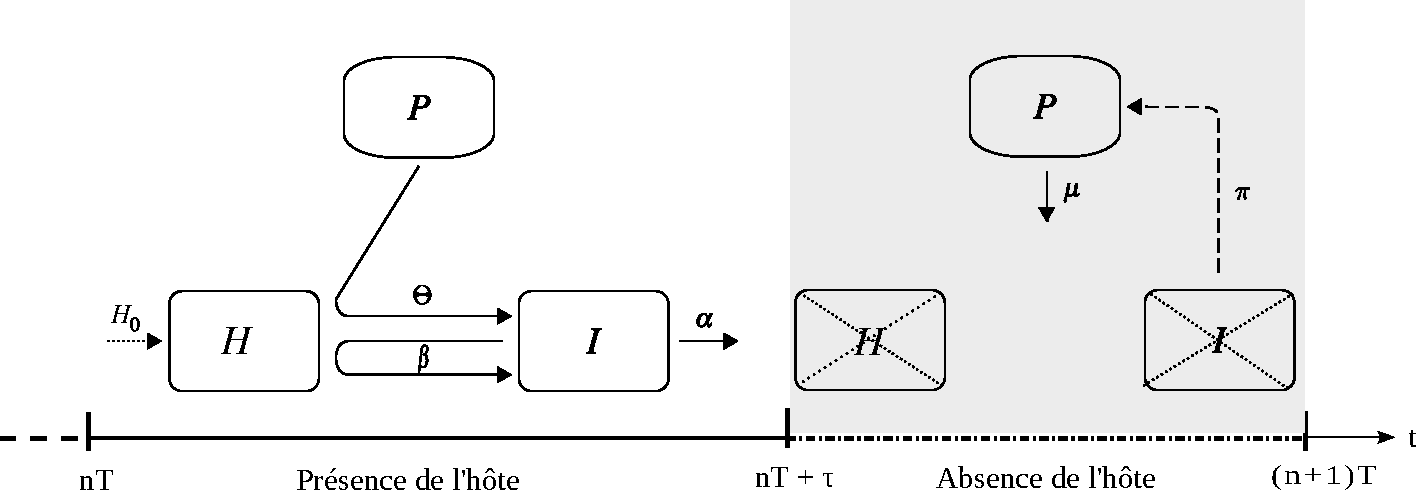
\includegraphics[width=1\linewidth]{Mailleret_semi-discrete}
		\caption[Diagramme du modèle épidémiologique semi-discret de \citet{Mailleret2012}]{Diagramme du modèle  
	    épidémiologique semi-discret de \citet{Mailleret2012}, correspondant aux équations~(\ref{eq:mailleret-saison}--
	    \ref{eq:mailleret-plant}). Deux périodes se succèdent pendant l'année de durée $T$ : 
	    la saison de culture, durant  laquelle la plante hôte est présente ($t \in (nT, nT + \tau])$ ; 
	    et la saison hivernale sans plante hôte $(t \in 
	    (nT + \tau, (n + 1)T])$. Le compartiment $P$ représente l'inoculum primaire (forme libre du pathogène), $H$ les 
	    plantes saines et $I$ les plantes infectées.
	    Les flèches pleines représentent les processus continus : infections primaires (taux $\Theta$) et secondaires 
	    (taux $\beta$), ainsi que mortalité liée à l’infection (taux $\alpha$) pendant la saison de culture ; mortalité 
	    de l'inoculum primaire (taux $\mu$) pendant la saison hivernale. Les flèches en pointillés représentent les 
	    processus discrets : plantation d’une nouvelle culture ($H_0$) au début de la saison de culture ; arrachage des 
	    plantes (ou perte des feuilles) et conversion des plantes infectées en inoculum primaire (taux $\pi$) au début 
	    de la saison hivernale. Adapté de \citet{Mailleret2012}. }
		\label{fig:mailleret}
	\end{figure}
	
	On considère, comme précédemment, la saison $n$, avec $n=0,1,\ldots$
\begin{enumerate}
\item \emph{Saison de culture, soit $t\in(nT^+,nT+\tau^-)$}\quad
La dégradation de l'inoculum primaire ($P$) pour un pathogène aérien (taux $\Lambda$) ou tellurique (taux densité-dépendant $\Xi$), les infections primaires (taux $\Theta$) et secondaires (taux $\beta$) des plantes saines ($H$), supposées densité-dépendantes, ainsi que  la mortalité (taux $\alpha$) des  plantes infectées ($I$) sont représentées : 
	\begin{equation}
	  \left\{
	    \begin{aligned}
	      \dot{P} &=
	      \left|
	      \begin{aligned}
	        &- \Lambda P &&\text{pathogène aérien} \\
	        &- \Xi P H &&\text{pathogène tellurique}
	      \end{aligned}
	      \right.\\
	      \dot{H} &= - (\Theta P  + \beta I) H,\\
	      \dot{I} &= + (\Theta P  + \beta I) H - \alpha I.
	    \end{aligned}
	  \right.
	  \label{eq:mailleret-saison}
	\end{equation}
	\item  \emph{Récolte, soit $t=nT+\tau$}\quad
	  À la fin de chaque saison de culture, les plantes sont arrachées (les feuilles des arbres tombent) et les débris de plantes infectées sont convertis en inoculum primaire (taux $\pi$) :
	  \begin{equation}
	    \left\{
	      \begin{aligned}
	        P(nT+ \tau^{+}) &= P(nT + \tau) + \pi I(nT + \tau),\\
	        H(nT+ \tau^{+}) &=0,   \\
	        I(nT+ \tau^{+}) &=0.
	      \end{aligned}
	    \right.
	    \label{eq:mailleret-recolte}
	  \end{equation} 
	\item  \emph{Saison hivernale, soit $t\in(nT+\tau^+,(n+1)T^-)$}\quad
	  L'hôte est absent et l'inoculum primaire se dégrade (taux $\mu$) :
	  \begin{equation}
	    \left\{
	      \begin{aligned}
	        \frac{dP}{dt} & = -\mu P, \\
	        H &= 0, \\
	        I~ &= 0. \\
	        \end{aligned}
	    \right.
	    \label{eq:mailleret-intersaison}
	\end{equation} 
	\item  \emph{Nouvelle saison, soit $t=(n+1)T$}\quad
	  Au début de la saison de culture suivante, de nouveaux hôtes sains sont plantés (les feuilles des arbres apparaissent) :
	  \begin{equation}
	   \left\{
	      \begin{aligned}
	        P((n+1)T^{+}) &= 0,\\
	        H((n+1)T^{+}) &= H_0, \\
	        I((n+1)T^{+}) &= 0.
	      \end{aligned}
	    \right.
	    \label{eq:mailleret-plant}
	  \end{equation}
	\end{enumerate}
		
	En supposant que les infections primaires sont rapides par rapport aux autres processus, les auteurs ont obtenu et étudié des modèles réduits \og compacts \fg{}, pour les pathogènes aérien et tellurique. Par ailleurs, ils se sont intéressés à la coexistence de deux souches de pathogène, en supposant qu'une souche est plus performante pendant la saison de culture (taux d'infection secondaire $\beta$ plus élevé) et l'autre pendant la saison hivernale (taux de mortalité $\mu$ plus faible). Ils ont montré que la coexistence des deux souches est possible pour le pathogène aérien, mais pas pour le pathogène tellurique, qui ne diffère du pathogène aérien que par la forme densité-dépendante du taux de dégradation de l'inoculum primaire. Ce résultat révise les conclusions de \citet{Vandenberg2010,Vandenberg2011}, qui sont fondés sur des modèles d'évolution en environnement saisonnier dans lesquels le principe d'exclusion compétitive\footnote{Principe d'exclusion compétitive (ou principe de Gause) : deux populations partageant la même niche écologique (\textit{e.g.} exploitant une ressource limitante unique) ne peuvent coexister indéfiniment.} s'applique.
	
	
\subsubsection{Hôtes résistants et  pathogènes virulents}
\label{sec:resist-virul}
	
	
	
	L'utilisation de variétés résistantes est un moyen de lutte à la fois efficace et respectueux de l'environnement (voir section \ref{sec:resistance} du chapitre \ref{intro}). Cependant, leur déploiement intensif peut mener à des contournements par des pathogènes virulents (voir section \ref{contournement} du chapitre \ref{intro}). Ainsi, différents travaux de modélisation se sont intéressés aux interactions entre plantes sensibles et résistantes, d'une part, et pathogènes avirulents et virulents, d'autre part, afin d'améliorer la durabilité des résistances ou le rendement des cultures \citep{vandenBosch2003,Fabre2012,Papaix2014,Fabre2015,Lof2017,Djidjou-Demasse2017}. 
Nous présentons ci-dessous plus en détails le modèle de \citet{Fabre2012} et son extension \citet{Djidjou-Demasse2017} qui sont aussi fondés sur un formalisme semi-discret.
	
	\citet{Fabre2012} ont recherché des stratégies de déploiement des plantes résistantes en fonction des caractéristiques du cultivar résistant, de l'aménagement du paysage et des pratiques culturales. Pour ce faire les auteurs ont développé un modèle décrivant la dynamique saisonnière d'une population de virus dans un paysage composé de culture résistantes et sensibles  dans une  mosaïque.
Pour  nombreux champignons ou nématodes phytoparasites, les virus responsables des maladies des plantes dépendent de leur hôte pour survivre et  la transmission du virus  a lieu lorsque les plantes  entrent en contact avec le virus ou via des vecteurs du virus. En cas d'absence de plantes cultivées, des réservoirs naturels (plantes sauvages, adventices) abritent le virus toute l'année, ainsi le virus peut donc survivre à l'hiver. L'infection primaire  démarre la phase épidémique. La propagation de la maladie est assurée par les infections secondaires : le virus se transmet aux plantes du même champ (auto-infection) ou  aux plantes des champs limitrophes (allo-infection).  Par conséquent, ces voies d'infection (i) entre le réservoir et les champs, (ii) entre les plantes du  même champ et (iii)  entre les plantes des autres champs peuvent éventuellement influencer les dynamiques des épidémies virales.
	
	Pour modéliser la saisonnalité des systèmes de culture, ils ont utilisé un modèle semi discret \citep{Mailleret2009}.  Ici, la partie continue est représenté par un modèle de type SI décrivant les dynamiques de transmission de l'infection de plantes à l'intérieur du même champ et  de plantes provenant d'autres champs.  Le paysage est composé de deux génotypes d'hôtes cultivés sensibles  et résistants   et deux variantes de virus avirulent  et virulent. Le cultivar sensible peut être infecté par les deux variants du virus. La plante résistante (porteuse de gènes R et impliquée dans une relation gène pour gène) peut être infectée uniquement par le variant virulent.  Le modèle permet de simuler l'épidémie d'une maladie virale pendant des années $y \in ([1,n_y])$ dans un paysage saisonnier et d'un réservoir de virus.  
		
	Nous décrivons d'abord le modèle dans un paysage composé uniquement de cultivar sensible. $\phi$ étant la proportion de champs composés de  plantes résistantes, ici $\phi = 0$.
	
	
	\begin{equation}
	\frac{I_{S,y}}{dt} = (n_p - I_{S,y})(\alpha_{E} + \beta_C (n_f -1) I_{S,y} + \beta_F I_{S,y})
	\label{sys4}
	\end{equation}
	
	
	Le compartiment $I_{S,y}$ représente  le nombre de plantes infectées dans un champ sensible donné au cours de l'année $y$. La taille de la population hôte est de $n_p$ plantes par champ. Le nombre de nouvelles infections par unité de temps est déterminé par le principe de l'action de masse entre les plantes saines et infectées, qui implique des contacts aléatoires entre les plantes.   Les épidémies virales se propagent dans une métapopulation d'hôtes composée de champs de taille $n_f$  et d'un réservoir.  Trois voies d'infection sont considérées dans ce paysage :  (i) entre le réservoir et les champs, (ii) entre les champs et (iii) à l'intérieur d'un champ. Les plantes saines $n_p - I_{S,y}$ peuvent contracter la maladie à partir des plantes  infectées $I_{S,y}$ dans le même champ à un taux de contact $\beta_F $ (unité : plante $^{-1} \cdot t^{-1}$)  ou à partir des plantes infectées dans les autres champs $(n_f -1) I_{S,y}$  à un taux de contact $\beta_C$ ( plante$^{-1} \cdot t^{-1}$).  Les plantes saines peuvent également contracter la maladie à partir de plantes infectées dans le compartiment du réservoir à un taux $\alpha_E$ (t$^{-1}$). La taille du réservoir n'est pas explicitement modélisée.
	
	Le modèle est étendu pour prendre en compte la proportion $\phi$ de champs cultivés composés de plantes résistantes : 
	\begin{align}
	\frac{I_{S,y}}{dt} &= (n_p - I_{S,y})\big[\alpha_{S,y} + \beta_C \big[((1-\phi)n_f -1) I_{S,y} + \phi n_f I_{R,y}\big] + \beta_F I_{S,y}\big] \label{sys5} \\ 
	\frac{I_{R,y}}{dt} &= (n_p - I_{R,y})\big[\alpha_{R,y} + \beta_C \big[(1-\phi)n_f \theta I_{S,y}) + (\phi n_f -1) I_{R,y} \big] + \beta_F I_{R,y}\big] \label{sys7} 
	\end{align}
	
	 Les équations \eqref{sys5} et \eqref{sys7}  permettent de prendre en compte les infections depuis les champs résistants vers les champs sensibles  et inversement. On sait que dans un champ composé de plantes résistantes seuls les variants virulents sont présents, tandis que dans les champs composés de plantes sensibles les variants virulents et avirulents dit \og sauvages \fg sont présents. Dans ce cas de figure, deux génotypes sont en compétition pour les ressources de la plante sensible. Dans l'équation \eqref{sys7}, le paramètres $\theta$ représente la fréquence de variants virulents qui coexistent avec le variant sauvage  à l'équilibre dans un champ ou parcelle composé uniquement de plantes sensibles. La fréquence de variants virulents à un équilibre de \og mutation-sélection \fg va dépendre du taux de mutation pour contourner la résistance et des coûts de fitness associés à l'acquisition de la virulence. Ce paramètre est donc un paramètre important car il représente les caractéristiques du gène de résistance.   
Durant l'hiver, la fréquence des variants au sein du  réservoir dépend de leur fréquence dans le paysage.
	
	Les auteurs ont étudié à partir de leur métrique pour différents scénarios épidémiologiques l'effet du ratio de plantes résistantes et des caractéristiques de la résistance. 
Ils ont conclu qu'il n'y a pas de stratégies universellement optimales (résistance pure \textit{vs} mosaïque).
 Les auteurs ont montré que l'intensité des épidémies jouait un rôle important sur les dommages relatifs et donc sur la  gestion de l'épidémie virale.
Lorsque l'intensité des épidémies était élevée et pour toutes les résistances testées une stratégie mosaïque était optimale.
Le choix du gène majeur de résistance (\textit{i.e.} le nombre de mutations nécessaires au contournement et le coût de fitness associé à chaque mutation dans les plantes sensibles) et le ratio de plantes est un facteur important dans la stratégie de déploiement de la résistance. Un ratio plus important  de plantes résistantes pouvait être déployé lorsque le gène de résistance était associé à de très forts coûts de fitness. En outre, dans le cas où la voie principale d'infection se faisait au niveau du réservoir une stratégie 100 \% résistant pouvait être optimale, parce que le réservoir hébergeait initialement très peu de variants virulents, ce qui entraîne peu d'infections de plantes résistantes. Par contre, lorsque les infections se faisaient principalement entre champs, des proportions intermédiaires de plantes résistantes étaient optimales. Ce résultat était possible grâce à l'effet de dilution qui tend à réduire les transmission de la maladie et donc la gravité des épidémies dans les mélanges de cultivars (voir sous sous section~\ref{durabilite_sub}.\ref{subsubsec:mel}). 
Cette étude a permis de démontrer l'importance des études numériques pour fournir des recommandations quant à un déploiement efficace et durable de la résistance à un virus en fonction des différents leviers d'actions des agriculteurs. Cette étude montre l'importance que constitue une stratégie mosaïques pour le contrôle d’une
maladie virale, en fonction des facteurs tels la connectivité entre les champs et réservoir et deux autres voies d'infections, l’intensité des épidémies et les caractéristiques du gène majeur de résistance. 
	
	\citet{Djidjou-Demasse2017} ont étendu ce modèle pour pouvoir considérer plusieurs gènes de résistance. Ils ont comparé les performances des stratégies de déploiement de deux à cinq gènes de résistance dans le paysage, obtenues soit en combinant les cultivars sensible et résistants monogéniques sous forme d'une mosaïque paysagère, soit en combinant les cultivars sensible et pyramidé. Ces stratégies faisaient intervenir des proportions prédéfinies ou optimisées des différents cultivars , ces proportions étant uniformes ou variables dans le temps.
Les auteurs ont conclu que les mosaïques étaient plus efficaces que le  pyramidage pour réduire les dommages causés par les pathogènes.
	
\section{Modèles appliqués aux nématodes des racines}
\label{sec:modeles-nematodes}
	
	Il existe différents  types de modèles dans la littérature. Tout d'abord, on retrouve ceux qui modélisent les dynamiques de populations à l’échelle d'un cycle cultural, qui représentent la grande majorité des approches. Ensuite, il existe  des modèles plus spécifiques qui s'attachent plus particulièrement à une phase du cycle de vie comme par exemple les modèles de survie hivernale \citep{Jeger1985, Starr1985, Jeger1993} . Enfin, plus rarement,  des  modèles multi-saisons qui permettent de développer un cadre de modélisation pour l'étude de stratégies de contrôle des nématodes  (\textit{e.g.} rotations, jachères, utilisation de pesticides) et/ou de leur évolution sur le long terme (\textit{e.g.} leur capacité à contourner un \gls{gene R}). 
	
	
\subsection{Une saison  de culture}
\label{sec:une-saison}
	
	
\subsubsection{Modèles de perte de rendement}
\label{sec:perte-de-rendements}
	
	Différentes équations ont été proposées pour mettre en relation la densité de population initiale de nématodes $P_i$ et le rendement de la culture $Y$ ou  le rendement relatif $y=\frac{Y}{Y_{max}}$, où $Y_{max}$ est le rendement attendu en l'absence de nématodes, notamment pour les nématodes à kystes de la pomme de terre (\textit{Globodera}) ou pour les nématodes à galles (\textit{Meloidogyne}).
	
	\citet{Brown1969} a effectué des régressions linéaires entre le rendement et le nombre initial d'œufs (avec ou sans transformation logarithmique) ou de kystes (avec ou sans transformation en racine carrée). \citet{Oostenbrink1966} a également utilisé un modèle de régression linéaire avec transformation logarithmique. %\stcom{Je n'ai pas ce dernier papier, à vérifier.}
	
	\citet{Seinhorst1965} a introduit une relation empirique entre rendement relatif ($y$) et densité initiale de nématodes ($P_i$), qui s'ajuste bien à des données expérimentales. Elle  est donnée  par cette équation :  
	\begin{equation}
	    \begin{cases}
	      y  =  m + (1-m)  z^{P_i-T} & \text{si }  P_i>T,  \\
	      y  = 1 &\text{si } P_i \leqslant T,
	    \end{cases}
	  \label{eq:Seinhorst1965}
	\end{equation}
où $P_i$ est la densité de population de nématodes dans le sol
au moment des semences ou de la plantation de la culture (exprimée en
œufs et/ou J2 par cm$^3$ ou g de sol) ; $T$ est la  tolérance, soit le seuil d'infestation initiale en dessous duquel aucun dommage n'est subi par la plante ;  $m$ est le ratio entre le rendement minimal à des valeurs très élevées de densité initiale de nématodes ($Pi  \rightarrow \infty$)  et le rendement maximal $Y_max$ (des valeurs de $m$ proches de 1 peuvent correspondre à un cultivar résistant) ; $y$ est le rendement relatif (le rendement à un
	 $P_i$ donné divisé par le rendement à $P_i$  $\leq$ $T$) ; et $z$ est une constante telle que $z<1$. \citet{Seinhorst1965,Seinhorst1970} a montré que $z^{-T}$  prend en général des valeurs entre $1$ et $1,15$.
	
	Ce modèle, qui a l'avantage d'être simple, a été utilisé surtout pour modéliser des
dommages causées par  une ou plusieurs générations de nématodes sur une
saison de culture. L'auteur l'a employé dans divers travaux \citep[par exemple]{Seinhorst1965,Seinhorst1970, Seinhorst1972, Seinhorst1986, Seinhorst1998}.
Dans la littérature,  de nombreux  travaux ont utilisé ce modèle  dans le  but de reproduire assez fidèlement des données issues d'expériences sur le terrain ou en conditions contrôlées ou semi-contrôlées. Une grande partie de ces travaux sont répertoriés  dans l'article  de  \citet{Greco2010}. Cet article fournit notamment les valeurs des paramètres  ($T$, $m$ et $z$) pour une grande variété de plantes et pour les espèces très préoccupantes du genre \textit{Meloidogyne}. Certains travaux sont repris ci-dessous.
	
	 \citet{Duncan1983} ont modélisé les effets des nématodes à galles \textit{Meloidogyne javanica} et \textit{M.~incognita} sur la croissance du niébé cv.~\textit{Californian Blackeye No.~5}  et ont montré que les dommages étaient plus importants avec \textit{M.~javanica} qu'avec \textit{M.~incognita}.  \citet{McSorley1992} ont montré  que l'effet de \textit{M.~arenaria} sur le rendement de l'arachide pouvait être modélisé efficacement à l'aide de ce modèle de Seinhorst~\eqref{eq:Seinhorst1965}. 
	%\stdel{Ils ont obtenu  comme valeurs de  paramètres : $T=1$ oeuf/100cm$^3$ de sol, $m=0,088$ et $z=0,90$.}
	
	\citet{Ehwaeti1998} ont mené une étude expérimentale pour examiner les dommages causés par
\textit{M.~incognita} à des  tomates, \textit{Lycopersicon esculentum}, cv.~\textit{Moneymaker} et ils ont mis en relation la densité initiale de  nématodes dans le sol avec un proxy de rendement relatif de tomates  à 42 et 135 jours de culture (\autoref{fig:Ehwaeti1998}). Cette approximation du rendement relatif est le ratio entre la biomasse racinaire  de tomates en présence et en absence de nématodes à 42 jours et à 135 jours après inoculation. De plus, ils ont ajusté leurs données expérimentales au  modèle de Seinhorst~\eqref{eq:Seinhorst1965}.
	%\stdel{Après 135 jours de culture, soit trois générations de nématodes, ils ont obtenu  comme estimation comme valeurs de  paramètres :$T =0,032$ œuf/g de sol, $z= 0,42$ et $m= 0,23$.}
	
	\begin{figure}[htp]
		\centering 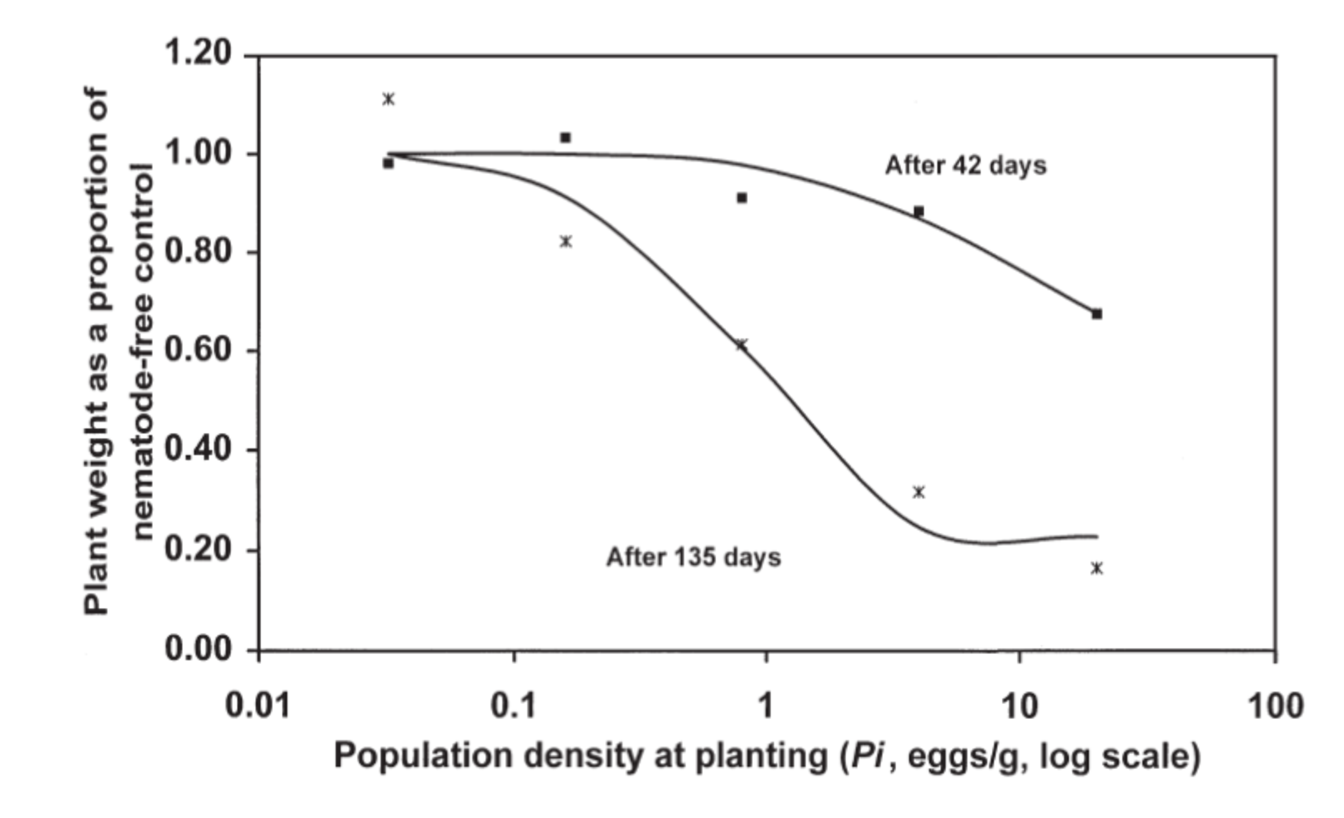
\includegraphics[width=1\linewidth]{ehwaeti2000-rendement.pdf}
		\caption[Rendement relatif de tomate en fonction des densités initiales de \textit{Meloidogyne incognita} dans le sol \citep{Ehwaeti1998}.]{Relation entre les densités initiales de populations  de nématodes \textit{Meloidogyne incognita} dans le sol et la biomasse relative de tomate (\textit{i.e.} ratio entre  biomasse racinaire  en présence et en absence de nématodes) à 42 et 135 jours post inoculation. Les courbes montrent l'ajustement au modèle de Seinhorst~\eqref{eq:Seinhorst1965}. D'après \citet{Ehwaeti1998,Ehwaeti2000}.}
		\label{fig:Ehwaeti1998}
	\end{figure}
		
	\citet{DiVito2004} ont modélisé la  relation entre les densités de populations initiales de \textit{M. incognita} et la perte de rendement du haricot cultivé en pots dans une serre (\autoref{Divito}).
	
\begin{figure}[hbtp]
\centering 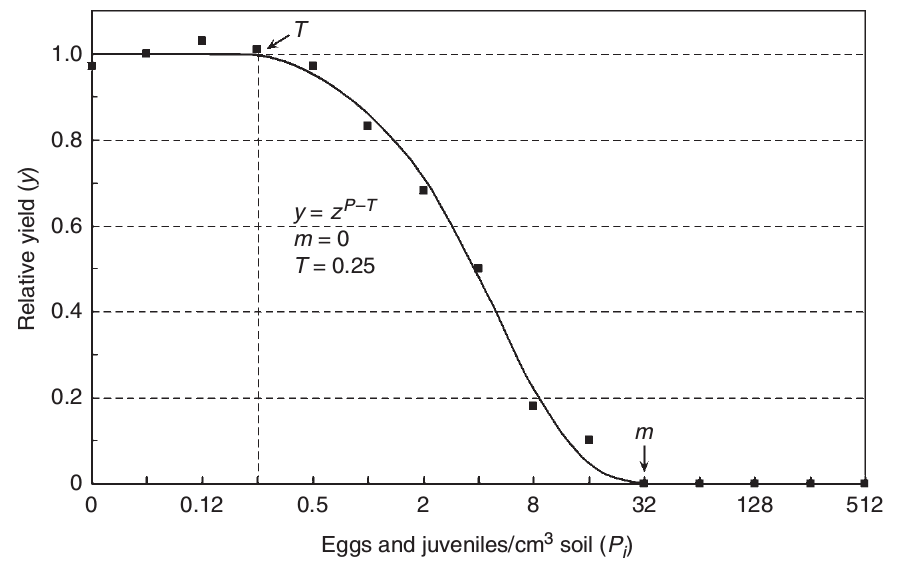
\includegraphics[width=1\linewidth]{Di_vito.png}
\caption[Rendement relatif de haricot en fonction des densités initiales de \textit{Meloidogyne incognita} dans le sol \citep{DiVito2004}.]{Relation entre les densités de populations initiales de \textit{Meloidogyne incognita} ($P_i$) et le rendement relatif ($y$) du haricot cultivé en pots dans une serre. Les courbes montrent l'ajustement au modèle de Seinhorst~\eqref{eq:Seinhorst1965}, les valeurs des paramètres $T$ et $m$ sont indiquées. D'après \citet{DiVito2004}.}
\label{Divito}
\end{figure}
	
	D'autres modèles ont été utilisés pour représenter la perte de rendement. \citet{Elston1991} ont étudié l'impact des nématodes à kystes de la pomme de terre (\textit{Globodera pallida}) sur cinq génotypes de pomme de terre partiellement résistant et un non résistant cultivés aux champs. Ils ont introduit un modèle linéaire inverse entre rendement relatif et densité initiale de nématodes : 
	\begin{equation}
		y = 1 - \frac{(1-m) P_i}{c + P_i}
		\label{eq:Elston1991}
	\end{equation}
	où $m$ correspond au paramètre du modèle de Seinhorst~\eqref{eq:Seinhorst1965}, soit le ratio entre le rendement minimal à des valeurs élevées de densité de nématodes et le rendement maxima sans nématodes, et $c$ est une constante. Dans cette étude, ils ont conclu que ce modèle alternatif pouvait décrire la perte de rendement avec moins de paramètres que le modèle de Seinhorst. 
	De plus, ils ont constaté que lorsque le paramètre $m$ était ramené à zéro,  cela ne nuisait pas à l'ajustement du modèle aux données.  Ils ont donc  proposé un modèle  plus simple encore, correspondant au modèle \eqref{eq:Elston1991} avec $m=0$ :
	\begin{equation}
		y =\frac{1}{1 + \frac{P_i}{c}}.
		\label{eq:Elston1991si}
	\end{equation}
	
	\medskip
	La plupart des modèles  de la littérature appliqués aux nématodes sont  des équations  qui relient les  populations finales de nématodes (\ref{eq:Seinhorst1966-migratory}--\ref{eq:Jones1978}) ou le rendement (\ref{eq:Seinhorst1965}--\ref{eq:Elston1991si}) aux populations initiales de nématodes sur une saison. Le seul paramètre ayant une  interprétation biologique claire est la tolérance $T$, \textit{i.e.} la faculté de l'hôte à tolérer le pathogène durant une saison de culture. 
	
	
	\subsubsection{Modèles de la dynamique des nématodes}
	
	Ces modèles relient les densités de nématodes en début et fin de saison de culture. Ils ont été introduits par \citet{Seinhorst1966,Seinhorst1967a,Seinhorst1967b,Seinhorst1967c,Seinhorst1970} et ont ensuite été largement repris.
	
	
	Cet auteur a utilisé le modèle logistique (voir Encadré~\ref{logistique}) pour représenter la dynamique des nématodes et relier la densité de population finale $P_f$ avec la densité de population initiale $P_i$ :
	\begin{equation}
	  P_f =  \frac{E_1 P_i e^{rt}}{ E_1 - P_i + P_i e^{rt}},
	  \label{eq:Seinhorst1966-migratory}
	\end{equation}
	
	où $e^{rt}$ est le nombre de descendants viables par femelle à l'instant $t$, avec $r$ le taux d'accroissement intrinsèque, et $E_1$ est la densité de nématodes à l'équilibre, soit la capacité de charge du modèle logistique (généralement notée $K$). 
	
	Ce modèle s'applique à la dynamique d'une large gamme de nématodes parasites des plantes. Cependant, il est plus approprié aux nématodes migrateurs (\textit{e.g.} l'ectoparasite \textit{Tylenchorhynchus dubius}), qui se multiplient continuellement pendant la croissance d'une culture hôte \citep{Seinhorst1970}. 
		
	Un autre type de modèle,  basé sur le modèle de compétition de
	\citet{Nicholson1935} et sur une courbe logistique,  décrivant la relation entre la densité initiale ($P_i$) dans le sol  et la densité finale ($P_f$) à  la fin d'une saison de culture a été proposé par  \citet{Seinhorst1967c,Seinhorst1970,Seinhorst1986} :
	\begin{equation}
		% P_f= a y\frac{ (1-q^{P_i})}{-{^e{log(q)}}} = y M  (1- e^{-x})
		P_f= a y\frac{ \left(1-q^{P_i}\right)}{-\ln(q)} = y M  \left(1- e^{-a P_i M^{-1} }\right)
		\label{eq:Seinhorst1970-sedentary}
	\end{equation}
	avec M = $a {(-\ln(q)})^{-1}$.
Dans cette   équation, $q<1$ est une constante très proche de 1  et peut être considérée comme la proportion de sites  potentiels pour le nématode ;
$a$ est le taux de multiplication maximum du nématode;  
$M$ est la densité de population maximale théorique en l'absence
de dommages ; et $y$ représente le rendement relatif. Le paramètre $P_i$ est généralement connu, il faut donc estimer les paramètres $M$, $y$ et $a$ grâce à des données issues d'études expérimentales bien réalisées. L'estimation du rendement relatif $y$ est obtenue par l'ajustement de données expérimentales au modèle de Seinhorst~\eqref{eq:Seinhorst1965} car le paramètre $y$  est généralement considéré comme le même $y$ dans les deux modèles de Seinhorst~ \eqref{eq:Seinhorst1965} et~\eqref{eq:Seinhorst1970-sedentary}. 
	
	\begin{encadre2}{Modèle de Verhulst}
	  \label{logistique}
	  En 1837, le biologiste belge Pierre-François Verhulst introduit le  modèle logistique en temps continu \citep{Verhulst1838} . Ce modèle permet de reproduire les dynamiques de nombreux macro- et micro-organismes. Il prend en compte  un processus d’autorégulation de la population observée, ou encore de compétition intra-spécifique pour les ressources (nourriture ou/et territoire) \citep{Brauer2012}.
	  Dans ce modèle, la dynamique de  la population  $P$ au cours du temps $t$ est donnée par :
	  \begin{equation*}
	    \left\{
	      \begin{aligned}
	        \dot{P}(t)&= rP(t) \left(1 - \frac{P(t)}{K}\right),\\
	        P(0)&= P_0,
	      \end{aligned}
	    \right.
	  \end{equation*}
où $r$ est le taux de croissance, $K$ la capacité de charge (\og carrying capacity \fg{} en anglais)  de la population et $P_0$ la taille initiale de la population. En intégrant cette équation, on trouve :
	  \begin{equation*}
	        P(t) = \frac{KP_0e^{rt} }{ K - P_0+ P_0 e^{rt}} = \frac{K}{1+\left(\frac{K}{P_0}-1\right) e^{-rt}} \quad  
	        \forall t \geqslant 0.
	  \end{equation*}
	 	La croissance logistique correspond à une croissance quasi exponentielle pour des faibles tailles de population, avec une saturation quand cette taille approche de la capacité de charge $K$. Cette dernière représente la taille de population maximale qui peut être maintenue de manière durable à partir des ressources disponibles.  Par ailleurs, l'équation logistique possède deux états d'équilibres :  $E_0 = 0$, qui correspond à une population éteinte,  et $E_1 = K$, la capacité de charge.
	\end{encadre2} 
	  
	  Selon \citet{Seinhorst1967a}, ce type de modèle~\eqref{eq:Seinhorst1970-sedentary} serait plus approprié pour les nématodes sédentaires, $eg.$ les nématodes à galles du genre \textit{Meloidogyne}. 
\citet{Ehwaeti1998} suite à leur étude expérimentale pour examiner les dommages causés par
\textit{M.~incognita} à des  tomates,  ont également mis en relation la densité initiale de  nématodes dans le sol avec leur densité finale à 135 jours de culture (\autoref{fig:Ehwaeti2000_ajustement_densite_finale}). De plus, ils ont ajusté leurs données expérimentales  au  modèle de Seinhorst~\eqref{eq:Seinhorst1970-sedentary}.
\begin{figure}[htp]
\centering 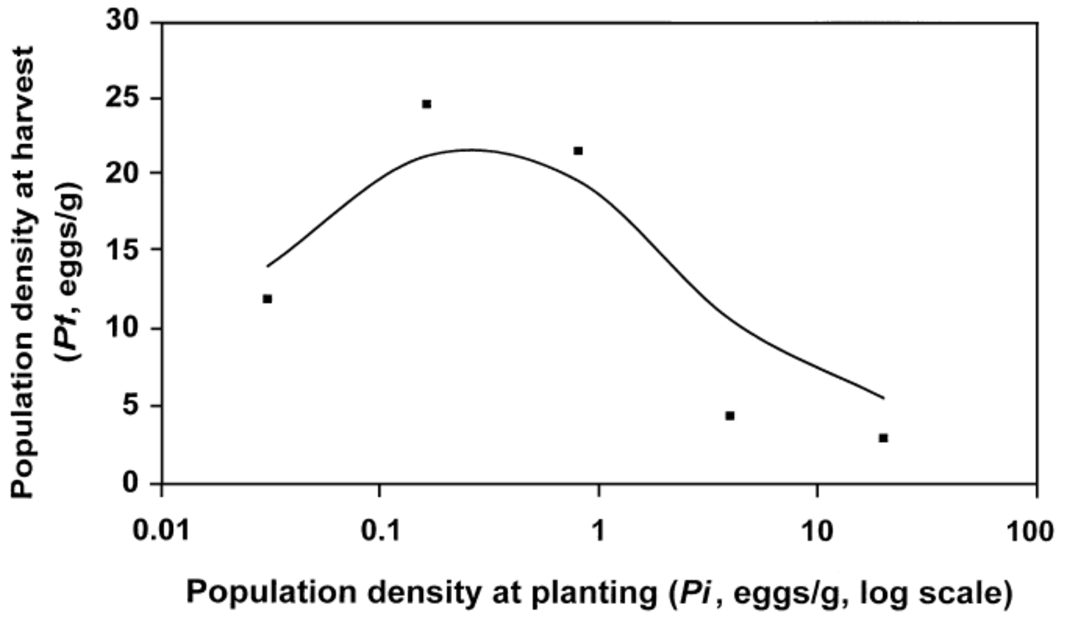
\includegraphics[width=1\linewidth]{Ehwaeti2000_ajustement_densite_finale}
\caption[Densités finales de \textit{Meloidogyne incognita}  en fonction de leurs densités initiales dans le sol à 135 jours de cultures post inoculation \citep{Ehwaeti1998}.]{Relation entre les densités de populations initiales et finales de nématodes \textit{Meloidogyne incognita}) à 135 jours post inoculation. La courbe montrent l'ajustement au modèle de Seinhorst~\eqref{eq:Seinhorst1970-sedentary}. D'après \citet{Ehwaeti1998,Ehwaeti2000}.}
\label{fig:Ehwaeti2000_ajustement_densite_finale}
\end{figure}
	
	
	
	
	En ce qui concerne les nématodes à kystes de la pomme de terre se nourrissant des racines de la pomme de terre deux formes de compétition sont présentes pour les ressources d'une plante (voir Encadré ~\ref{competition}). Il y a un nombre maximum de sites nourriciers par unité de poids de racines de la pomme de terre pour nourrir un nématode femelle (\textit{contest competition}). En outre, les nématodes femelles s'alimentant au niveau d'un site nourricier de manière égale pour se reproduire conduit à une diminution des ressources de la plante (\textit{scramble competition}). 
Des  considérations plus spécifiques sur la biologie des nématodes à kystes de la pomme de terre  ont été prises en compte dans le modèle de \citet{Jones1978b}  pour relier les densités finales de nématodes $(P_f)$ en fonction de leurs densités initiales  $(P_i)$ : 
	
\begin{equation}
	  P_f  = \frac{e^{rt} H P_i}{1 + \frac{b H P_i}{h} }= \frac{P_i}{\frac{1}{e^{rt} H} + \frac{bP_i}{h e^{rt}} }
	  \label{eq:Jones1978}
\end{equation}
où  $h$ est la densité de racines dans le sol ; $H$ est la proportion de juvéniles viables qui s'installent avec  
succès dans les racines ; $b$ est le ratio de mâles par rapport aux nombres de femelles dans la population ; et  
$e^{rt}$ est le  nombre moyen d’œufs produits par une femelle, avec $r$  le taux d'accroissement intrinsèque. . 
	
	L'équation~\eqref{eq:Jones1978} a aussi été modifiée pour introduire la compétition intraspécifique, en considérant $h$ comme une fonction décroissante  de la densité initiale de nématodes dans le sol $P_i$. Ainsi, la densité finale de nématodes dans le sol décroît avec les fortes valeurs de $P_i$ à cause de la compétition pour les ressources de la plante. 
	
	
	\begin{encadre2}{La compétition}
	\label{competition}La compétition pour les ressources est l’une des principales interactions écologiques essentielles dans la régulation des populations et des communautés. Elle est définie comme une interaction entre espèces vivantes dans laquelle les performances d’un individu en termes de reproduction, de croissance ou de survie, sont réduites par la présence d’autres espèces.  La compétition peut intervenir aussi bien entre des individus d’espèces différentes (compétition inter-spécifique) qu’au sein d’une population d’individus de la même espèce (compétition intra-spécifique).  Deux formes de compétitions, suggérées  par \citet{Nicholson1954}, traduisent la manière dont les ressources sont réparties entre les individus : i) la compétition par exploitation (\textit{scramble competition}) et ii) la compétition par interférence   (\textit{contest competition}). Pour la compétition par exploitation, la ressource limitante  est partagée de manière égale entre les compétiteurs, de telle sorte que la quantité de nourriture par individu diminue avec l'augmentation de la densité de population. De ce fait, la compétition par exploitation est  une forme de compétition où les individus ont un effet négatif les uns sur les autres en consommant une ressource limitante.  Cette forme de  compétition est  dite indirecte car elle ne requiert pas d’interaction directe entre les individus.  La compétition par exploitation est répandue et a été introduite par le modèle logistique (voir Encadré~\ref{logistique}).
	 \par\medskip
	  A l’inverse, il existe une autre forme de compétition appelée compétition par interférence.  Dans ce cas,  les compétiteurs les plus forts obtiennent  les ressources trophiques dont ils ont besoin pour survivre ou se reproduire au détriment des plus faibles. Ils réduisent les performances des compétiteurs dominés (les plus faibles)  en accaparant partiellement ou totalement l’accès à la ressource convoitée. Cette ressource peut être une source d’alimentation, un habitat ou un partenaire sexuel.  
	\end{encadre2}
	
	%\stdel{Un des avantages de cette  nouvelle équation est qu'elle prend en compte davantage le cycle de vie du nématode. En effet, après avoir pénétré dans l'hôte, le nématode à kyste  s'installe pour se nourrir au centre d'une jeune racine. L'alimentation induit le développement de cellules géantes qui interrompent l'activité vasculaire normale dans la racine. Ainsi il est important de prendre en compte l'impact de la densité de nématodes sur la biomasse racinaire. \stcom{Le cycle de vie du nématode n'apparaît pas clairement pour moi dans l'équation ci-dessus. $h$ qui décroît avec $P_i$, est-ce de la compétition ou alors l'impact de la densité de nématodes sur la biomasse racinaire ? }}
	 %Certains des nématodes se transforment en petits mâles semblables à des vers qui finissent par s'échapper dans le sol. Après la reproduction, les femelles meurent et leur corps se transforme en kystes protecteurs à parois dures, remplis d'œufs minuscules et ovales. Ces kystes finissent par se retrouver dans le sol et éclosent qu'au contact d'exsudat induit par les racines des plantes (Abad2010). Les oeufs peuvent rester dans le sol pendant des années avant d'éclore. Ce type de modélisation  plus réaliste est un  bon cadre  pour refléter l'intensité d'une épidémie causé par des parasite telluriques et constitue donc une référence pour la modélisation de maladies telluriques à l'échelle d'une saison de culture.
	
	%Par ailleurs, Jeger and Strarr  \citep{Jeger1985} ont développé  un modèle théorique de la dynamique de la survie hivernale des nématodes à galles (\textit{Meloidogyne spp.}) 
	%en considérant le rôle de l'éclosion des œufs et de la mortalité des juvéniles (J2) sous formes libres en absence de l'hôte pendant l'hiver.
	%Dans la suite nous aborderons les modèles qui se sont intéressés  à l'impact des densités initiales de nématodes dans le sol sur le rendement de la plante. 
	
	
\subsection{Modèle de survie hivernale}
\label{sec:modele-intersaison}
	
	La survie des nématodes varient selon les facteurs biotiques (biologie des nématodes, présence ou absence des hôtes, présence d'autres espèces dans le milieu) et abiotiques (température, sol)  \citep{Bergeson1968, Abad2010, Perry2009}. Ces conditions sont elles mêmes sujets aux variations notamment à cause des conditions  environnementales (e.g. hiver) et plantes cultivées qui diffèrent d'une parcelle, ou d'une exploitation à l'autre (e.g plantes annuelles) ce qui  affectent d'autant plus la survie des nématodes phytoparasites.   
\citet{Jeger1985} ont développé  un modèle théorique de la dynamique de la survie hivernale des nématodes à galles (\textit{Meloidogyne spp.}) 
en considérant le rôle de l'éclosion des œufs et de la mortalité des juvéniles (J2) sous forme libre en absence de l'hôte pendant l'hiver. Chez l'espèce \textit{Meloidogyne}, 
les femelles peuvent produire des œufs pendant deux à trois \citep{DeGuiran1983}. Sous  conditions  favorables  d’humidité  et de températures, la plupart des œufs éclosent immédiatement et évoluent en larves.  Lorsque  les  conditions  sont  peu  favorables,  ils  peuvent  passer  sous  une  forme  de  résistance  et  survivre  plusieurs années    dans  le  sol  \citep{DeGuiran1983}. La  température  du  sol  est  primordiale  en  dessous  de  12  $^\circ$C  et  au­ dessus  de  22  $^\circ$C,  les  juvéniles  se  déplacent  difficilement  \citep{Vrain1978}.  Entre  0  et  5 $^\circ$ C,  les  juvéniles  survivent  pendant  sept jours mais ne sont plus infectants, et  meurent  en  vingt  jours  \citep{Vrain1978, Tsai2008}.  L’existence d'une telle  survie des nématodes sous des conditions défavorables justifie que l'auteur utilise un modèle plus mécaniste dont les variables ou les populations  sont décrites par des équations différentielles ordinaires plutôt qu'une équation discrète. Ce modèle a été repris dans d'autres études \citep{Starr1985, Jeger1993}. 

	
\subsection{Plusieurs saisons de cultures}
\label{sec:plusieurs-saisons}
	
	 La  dépendance d'une année à l'autre des densités de populations de nématodes phytoparasites  à un endroit donné est importante. De ce fait, le nombre de nématodes d'une espèce donnée  dans le sol l'année suivante est déterminé par des stratégies de gestion qui ont été mises en place  pour éviter des dommages aux cultures et la multiplication des nématodes l'année précédente \citep{Seinhorst1970}.   À travers des modèles mathématiques, il est possible de suivre les densités de populations des nématodes et d'étudier comment ces populations sont affectées dans le temps par la mise en place de ces stratégies de gestion.
Les rotations de cultures (de variétés ou d'espèces) sont considérées comme l'une des meilleures stratégies de contrôle des nématodes. Les modèles de rotation des cultures sont variés et dépendent du cadre de modélisation utilisé. Il s’agit par exemple de modèles de programmation linéaire ou de modèle statistiques ou dynamiques.  Ces cadres de  modélisation généralement proposent une gestion optimale des nématodes phytoparasites par des stratégies permettant le maintien des densités de nématodes sous un seuil de nuisibilité et  augmenter les rendements des cultures.
	%Selon la théorie, la  dépendance d'une année à l'autre des densités de population de nématodes phytoparasites  à un endroit donné est importante, $ i.e$ le nombre de nématodes d'une espèce donnée  présent dans le sol l'année suivante est déterminé par les stratégies de gestion qui ont été mise en place  pour éviter des dommages aux cultures et la multiplication des nématodes l'année précédente (\citep{Seinhorst1970}). 
	
	
\subsubsection{Modèle de programmation linéaire}
	
	 De nombreux modèles de rotation ont utilisé un cadre de programmation linéaire. La programmation linéaire offre un moyen pratique et efficace  de modéliser les relations entre des séquences de cultures sur une période de plusieurs années. \citet{Taylor1999} ont utilisé la programmation dynamique stochastique pour maximiser le profit  attendu des séquences de rotations  d'arachides et de coton pour le contrôle épidémique du nématode à galle, \textit{Meloidogyne  arenaria}. Une vue d'ensemble plus complète de l’utilisation des modèles de rotations grâce à la programmation linéaire est disponible dans l'excellente review de \citep{Dury2012}.  Nous ne rentrerons pas plus en profondeur dans cette thématique car nous nous sommes plus particulièrement intéressés dans cette thèse aux modèles dynamiques.
	
	
\subsubsection{Modèles statistiques ou dynamiques}

	  \citet{Kinloch1986} a proposé un modèle  pour décrire l'influence des rotations des cultivars de soja et de maïs  sur les densités de  \textit{M. incognita} dans le sol.
La dépendance des densités de nématodes d'une année à l'autre en même endroit rend la dimension temporelle très importante.  Des données sur la rotation des cultures ont été collectées de 1972 à 1980 sur un site infesté par \textit{M. incognita} en Floride.  Les cultures d'été consistaient à des cultivars de soja sensibles ou résistants contre M. \textit{incognita} cultivés soit en monoculture, soit en rotation avec du maïs. Pendant les mois d'hiver une jachère était mise en place. À la fin de chaque saison de culture (en novembre), toutes les parcelles étaient échantillonnées afin de déterminer les densités de nématodes dans le sol (juvéniles de deuxième stade). Les auteurs ont mis en relation la densité de nématodes de l'année ($Y$) en fonction de la densité  de nématodes de l'année précédente ($X$), et en fonction des cultures précédant les deux mesures (\autoref{fig:XY}).
	
	\begin{figure}[H]		
		\centering	
		    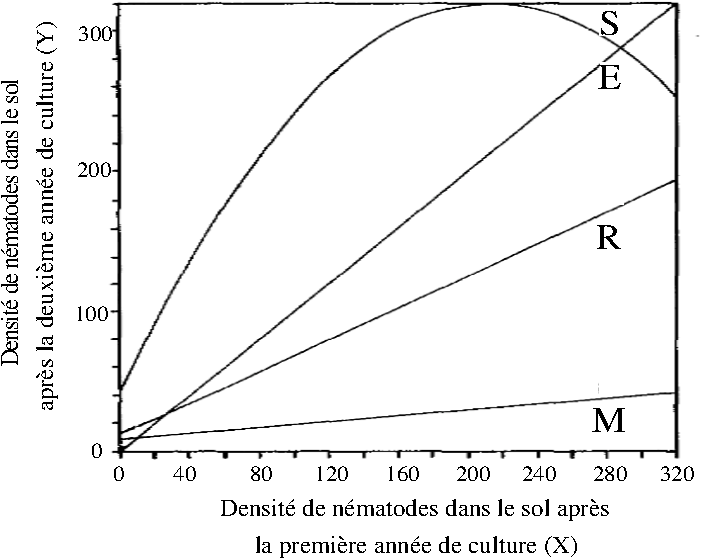
\includegraphics[width=0.6\linewidth]{multisaisXY.pdf}
			\caption[
			Relations entre les populations de nématodes \textit{Meloidogyne incognita} après récolte   au cours de  
			deux années successives de plantation.]{
			Relations entre les populations de nématodes \textit{Meloidogyne incognita} après récolte au cours de deux 
			années successives de plantation de soja sensible (S), $Y = 44,919 + 2,5667X - 0,006X^2$; de soja résistant 
			($R$); de maïs ($M$). $E$ représente la droite $Y=X$.
			\label{fig:XY}}
	\end{figure}
	
	 L'influence de  différentes séquences de rotation sur la densité de nématodes après la récolte a été simulée dans cet article.  
L'auteur a  évalué plusieurs séquences  pour la gestion  des  nématodes \textit{Meloidogyne incognita} en rotation des cultures et a conclu qu'une rotation occasionnelle avec du maïs ou tous autres cultures mauvais hôtes avec des hôtes résistants pourrait être une solution efficace  pour la gestion de \textit{Meloidogyne incognita}.
	
	\citet{Vandenberg2005}, ont modélisé la dynamique de  populations des  nématodes endoparasites migrateurs des racines  (\textit{Pratylenchus penetrans}) et la perte de rendements d'un système de culture, basé sur l'alternance  de différentes cultures hôtes  et de jachères. Ils ont examiné en tout 6 rotations de cultures  différentes.
Pour modéliser la dynamique des nématodes sur plusieurs saisons, les auteurs ont mis en relation la densité finale après la récolte, $P_f$  avec la densité initiale de nématode  avant que la culture ne soit plantée ou semée,  $P_i$  :
	
	 \begin{equation}
	        P_f = \frac{P_i}{ \alpha + \beta P_i},
	        \label{sys2}
	 \end{equation}
	 
\noindent{où} $\frac{1}{\alpha}$ représente la pente de la courbe à l'origine et $\frac{1}{\beta}$ représente l'asymptote horizontale de la courbe. On peut remarquer que la structure
de l'équation~\eqref{eq:Seinhorst1966-migratory} dans la  section~\ref{sec:une-saison} est similaire à l'équation~\eqref{sys2} en posant $\frac{1}{e^{rt}}= \alpha$ et $\beta$  égale à $(e^{rt}-1)/e^{rt}E_1$ et en réécrivant l’équation ~\eqref{eq:Seinhorst1966-migratory} sous cette forme :
	
	\begin{equation}
	  P_f =  \dfrac{P_i}{  \frac{1}{e^{rt}} + \dfrac{(e^{rt}-1)}{e^{rt}E_1}P_i},
	  \label{eq:Seinhorst1966-migratory}
	\end{equation}
	
	
	En partant de l'équation~\eqref{sys2} et en prenant $\beta=0$ les auteurs ont pu estimer la survie du nématode à l'intersaison par l'équation :
	\begin{equation}
		P_f=\frac{1}{\alpha} P_i.
		\label{survie} 
	\end{equation}
	
	
	\noindent{où} $\frac{1}{\alpha}$ en termes d'interprétation biologique correspond à la probabilité de  survie en absence de l'hôte. L'intersaison correspond à une période sans culture hôte dans laquelle une culture non hôte peut être présente ou une jachère peut être mise en place. %  L'équation~\ref{survie}  est également pertinente pour estimer la fraction du nématode %population qui survit à une mesure de contrôle \citep{Vandenberg2005}.
	
	En second lieu, toujours à partir de la structure du système \eqref{sys2} ils ont  développé un modèle dynamique saisonnier pour le contrôle d'une seule espèce de nématode qui interagit avec plus d'une culture hôte dans la rotation \footnote{Dans une rotation, $n$ cultures sont cultivées pendant $n$ année. Chaque culture est considérée comme une phase de la rotation, la culture $1$ étant phase $1$, la culture $2$ étant la phase $2$ et ainsi de suite.}. La dynamique des densités de populations de nématodes $P(t)$  au début de l'année $t$ dans une rotation de $n$ cultures est la suivante :
	
	
	$$
	 \left.
	    \begin{array}{ll}
	        P_{t+1} =&   \frac{P_t}{\alpha (\tau (t)) + \beta (\tau(t))} \\
	  
	    \end{array}
	\right \} P_1= \pi_0,
	$$
	
	dans laquelle $\tau(t)=t(\text{mod})n$. La fonction $t(\text{mod})n$ est telle que $t$ est égale à $1$ à l'année $1$, égale à $2$ à l'année $2$, égale à $n$ à l'année $n$ et à nouveau égal à $1$ à l'année $n+1$, égale à $2$ à l'année $n+2$ ainsi de suite. La densité de nématodes avant la première culture, $0$, dans un champ est un
paramètre spécifique du modèle. Les paramètres $ \alpha(\tau(t))$ et $\beta(\tau(t))$ dépendent
de la culture cultivée au cours  de l'année $t(\text{mod})n$.
Les expressions analytiques pour
les états stables  de ce modèle dynamique ont été obtenues et démontrées. La dynamique des populations
est combinée avec un modèle d'évaluation de la perte de rendement pour permettre l'évaluation des
rendement financiers \footnote{Le modèle de rendement financier s'inspire du modèle de rendement présenté \eqref{eq:Elston1991si}} associés. Pour plus de détails sur le modèle de pertes de rendements économiques et le calcul des états d'équilibres voir \citet{vandenberg2011b}.
	
	 Le modèle a été ajusté à des données pluri-annuelles d'un système de culture adapté à la gestion des nématodes \textit{Pratylenchus penetrans} avec des traitements divers au cours des saisons.   L'estimation des paramètres de ce modèle multi-saisons pour chaque type de culture dans la rotation a été effectuée à l'aide de statistiques bayésiennes telles que les chaînes de Markov Monte Carlo (MCMC). Les auteurs ont étudié
un cas où la même équation s'applique à chacune des cultures, et les différences entre
les cultures sont prises en compte uniquement dans les estimations des paramètres.
En termes de cas d'étude, les auteurs ont  évalué six rotations de quatre ans comprenant trois types de cultures (laitues, carottes, poireaux  et une seule période de jachère \footnote{Par exemple une rotation peut ressembler à une succession chaque année de laitues-poireaux-carottes-jachère. La première année l'agriculteur cultive des laitues, la seconde année des carottes, la troisième année des poireaux et la quatrième année une jachère}). Pour chaque rotation, les densités de \textit{Pratylenchus penetrans} avant la plantation de chacune des quatre cultures, ont été calculées à l'état d'équilibre. Pour chaque culture dans chaque rotation, le rendement et la production financière ont été calculés, ainsi que le rendement   moyen financier par rotation.   Ce cadre de modélisation spécifique repose sur la calibration  des paramètres (du modèle dynamique) grâce à une quantité très importante de données expérimentales et l’utilisation de modèles statistiques complexes.
	En partant de cette structuration de modèle d'autres auteurs ont proposé des modèles saisonniers de la même structure \citep{Ferris1992, Burt1996}.
	
	Dans la littérature, on retrouve rarement d'autres types de modèles à l’échelle  de plusieurs saisons de culture dans le cas des nématodes phytoparasites ou des racines. Après avoir réalisé un état des lieux sur les modèles existants appliqués aux nématodes à galles, nous avons pu constater que les rares  modèles  qui existent et qui décrivent la dynamique des nématodes  des racines sur le  long terme dans des rotations de cultures  sont basés sur le long terme dans des rotations de cultures sont basés sur des modèles statistiques ou dynamiques.  
Le modèle de \citet{Vandenberg2005}  a presque une structure que nous pourrions utiliser pour modéliser la dynamique des nématodes sur plusieurs saisons.  Par exemple, ce modèle repose principalement sur des équations discrètes, une qui relie le début et la fin de la saison et une qui décrit la survie du nématode.   
Toutefois, le modèle de  \citet{Vandenberg2005} qui modélise un seul génotype de plantes sensibles et de nématodes avirulents ne  permet pas d'étendre ce cadre de modélisation à d'autres génotypes de nématodes et de plantes. Effectivement, il est peu adaptable par son manque de description plus fines des processus biologiques qui régissent l’interaction plante-nématode durant la phase épidémique. 
	
	Dans notre étude, il était important pour nous de bien décrire finement les processus biologiques de l’interaction hôte-nématode  par rapport à ce que nous voulions faire. Nous avions dans premier temps le but de rechercher des stratégies de rotation entre cultivars de plantes sensibles et résistantes permettant une meilleur gestion  des nématodes à galles. Ces stratégies de rotations de cultivars sensibles et résistants sont connues (surtout pour d'autres pathosystèmes) pour permettre de limiter les risques de contournement des résistances des plantes et d'augmenter le rendement des cultures en jouant sur les pressions sélectives.  De fait, il était important pour nous d'avoir un cadre de modélisation permettant de suivre et de comprendre comment i) les dynamiques de populations de nématodes (avirulents et virulents) sont affectées par l'alternance de pressions sélectives dans le temps et ii) de leur impact sur le rendement des cultures. 
Chez les nématodes à galles, l'acquisition de la virulence s'octroie au prix de  coûts de virulence sur le taux de  reproduction et d'infection. Ainsi, les nématodes virulents sont sélectionnés en cas d'usage de plantes
résistantes, mais ils sont contre-sélectionnés en cas d'usage de plantes sensibles au profit
de nématodes avirulents à cause d'une moindre fitness.
L’intensité des pressions sélectives  dépend des différences des traits  d'histoire de vie entre les compétiteurs (taux reproduction, capacité d'infection et des éventuelles coût de virulence). Pour décrire précisément ses effets sur la dynamique de la population, il était donc nécessaire d’adopter une approche plus mécanistique qui permet de décrire plus finement les processus biologiques de l'interaction plante-nématode et d'étendre notre modélisation aux cas virulents/avirulents. 
	Les systèmes dynamiques de modèles semi-discrets pourraient permettre  de décrire, suivre et de comprendre   comment les changements de cultivars hôtes  pendant la phase épidémique  et la phase de survie (\textit{i.e.} absence d'hôte, mauvais hôte) influencent successivement les  dynamiques de populations des nématodes \footnote{la
variation du nombre de nématodes dans le temps
est définie comme étant une dynamique de la population}  sur plusieurs saisons de cultures. Puisque ces modèles semi-discrets intègrent explicitement les processus biologiques comme l'infection et la reproduction,   ils rendent possible l’intégration  des coûts de virulence et de la mutation en fonction des caractéristiques de la résistance dans notre étude. La compréhension de la biologie du nématode et l'utilisation de modèles mécanistes saisonniers  sont des atouts majeurs pour permettre la recherche de stratégies de gestion bien adaptées aux nématodes des racines sur le long terme.
	 
	 
	
	
	
	\subsubsection{Modèles mécanistes du type PHI, PHEI et saisonnalité}
	La littérature est quasiment exempte de modèles mathématiques mécanistes saisonniers rattachés de manière très concrète à des processus biologiques appliqués aux
nématodes des racines dans les agrosystèmes actuels. Par exemple, un des seuls modèles a été conçu
par \citet{Tankam-Chedjou2020}  dans le cadre de l’équipe associée Cameroun-France EPITAG de l’Inria. Ils  ont développé  un modèle  multi-saison pour le contrôle épidémique des nématodes foreurs des racines de la banane plantain \textit{Radopholus simili}. Le nématode de la famille des \textit{Pratylenchidae}, \textit{Radopholus similis} est un parasite obligatoire qui  se nourrit que de racines fraîches et induit une nécrose au niveau des  racines. On le trouve principalement dans les racines et les rhizomes, et peu dans le sol. Lorsqu'il infecte des racines fonctionnelles, \textit{Radopholus similis} creuse les tissus en se nourrissant. Les femelles pondent quatre à cinq oeufs par jour pendant deux semaines dans les zones de nécrose des racines. Les juvéniles restent alors soit dans la racine et creusent un terrier pour se nourrir de tissus frais, soit ils partent et migrent dans le sol pour trouver une autre racine.
Cette étude repose  sur l’utilisation de modèles semi-discrets, dans lesquels la partie en temps continu modélise les interactions entre les nématodes et les plantes au cours de la saison. La partie en temps discret est similaire au modèle de \citet{Hamelin2011} ou de  \citet{Mailleret2012} et de permet  décrire le passage à l'interculture, soit à une jachère ou une culture non hôte (voir section~\ref{sec:ext}.\ref{sec:sais}).  C'est un modèle qui a été conçu  pour un nématode en particulier qui diffère  en termes de biologie et de stratégies de contrôle par rapport au modèle d'étude de cette thèse, le nématode M. \textit{incognita}.
	 Le modèle de  \citet{Tankam-Chedjou2020} permet effectivement de modéliser la  partie continue de l’interaction hôte-parasite  par un modèle mécaniste du type \og PHI \fg . 
	
	 En revanche, ce modèle ne prend pas en compte la période de latence ($E$) très importante dans le processus  biologique du nématode  \textit{M.~incognita}. Par ailleurs, une autre caractéristique typique
dans les agrosystèmes au delà la saisonnalité est la résistance génétique des plantes. La littérature est quasiment exempte de modèles décrivant l'évolution de populations de nématodes en réponse à des variations de qualité d'hôtes au cours du temps telle que les alternances de variétés résistantes et sensibles, notamment pour les nématodes des racines. Ces variations sont connues pour influer considérablement sur l'adaptation des populations parasites en général \citep{Crossan2007, McDonald2002, Zhan2015} et l'évolution de la virulence chez les nématodes après l'introduction de la résistance génétique des plantes  \citep{Castagnone-Sereno2002}. 
	Par une approche similaire au modèle de~\citet{Tankam-Chedjou2020},  nous avons développé en mème temps dans des groupes de travail proches, un modèle épidémiologique semi-discret pour le contrôle des nématodes à galles. À notre connaissance, aucune étude n'a élaboré un modèle prenant en compte la spécificité des nématodes  \textit{M.~incognita}  à forme libre, peu mobiles, enchaînant phases de
développement sur le chevelu racinaire de plantes (sensibles ou résistantes) et phases de survie dans le sol (influencés par des pratiques  agricoles, l'absence d'hôtes ou présence de mauvais hôtes).  Pour palier à ce manque dans la littérature, nous avons développé un modèle décrivant la dynamique de populations des nématodes selon un formalisme semi discret \citep{Madden2002, Mailleret2012}.  Ce cadre de modélisation serait particulièrement intéressant pour étudier de manière numérique  les dynamiques  qui régissent l'interaction hôte - nématodes à galles et pourrait être un cadre très convaincant pour développer des stratégies de gestion des résistances et augmenter les rendements sur le long terme.  
	
	
	 
	
\section{Notre stratégie de modélisation}\label{sec:notre-strategie}

\subsection{Nos hypothèses} \label{sec:nos-hypotheses}
	
	Nous avons choisi de décrire la dynamique d’une population de nématodes dans les racines
d’une plante comme une épidémie de parasites à forme libre se développant sur un chevelu racinaire en croissance.
Le cadre de modélisation que nous avons choisi s'appuie sur un formalisme du type semi-discret  et permet de suivre  la dynamique des formes de vie libres du parasite pendant les épidémies saisonnières \citep{Madden2002, Hamelin2011, Mailleret2012}. Pour prendre en compte la période de développement du nématode juvénile en une femelle mature, cela nécessite l'ajout  de la période de latence qui correspond à  un compartiment $E$ (section~\ref{sec:ext}.\ref{sec:latence}) dans le modèle  PHI (section~\ref{sec:ext}.\ref{sec:libres}). L'unité élémentaire racinaire  correspond  à un site nourricier potentiel pour un nématode.  On considère que le chevelu racinaire est composé de sites potentiellement hôtes pour une femelle, c'est pour cela que nous parlons de sites nourriciers potentiels. Ainsi, \og un site \fg{} correspond à une quantité de racine nécessaire pour établir 1 site nourricier pour 1 nématode. 
		 
	Tout d'abord, nous ne considérons que les interactions entre nématodes avirulents  et une plante sensible.
	On introduit l'indice $_a$ se réfère aux populations de nématodes avirulents et l'exposant $^X$  indique le type de plante cultivée dans la saison culturale en cours, ici une plante sensible (exposant $^S$).  Dans ce  modèle,  les variables  représentent quatre compartiments : les densités de nématodes avirulents libres   dans le sol ($P_a$), les densités de racines  saines d'une plante sensible  ($H^S$), les  densités de sites nourriciers infectés  de manière latente ($E_a$) et infectieuse ($I_a$)  par les nématodes avirulents. Nous représentons le modèle 
compartimental dans un diagramme de transmission d’une infection entre la population de nématodes avirulents et la 
population de plantes sensibles au sein d’une saison de culture (\autoref{fig:mod-planteS-nemavr}) :



	\begin{figure}[H]	
		\centering	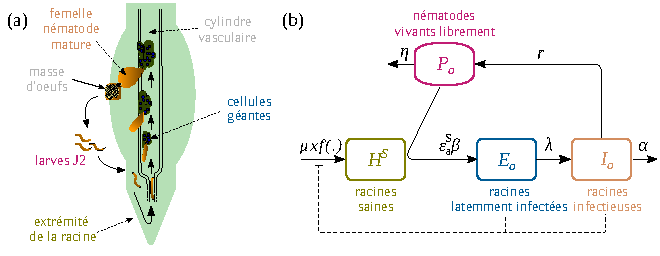
\includegraphics[width=1\linewidth]{mod_avirulent_planteS.pdf}
		 \caption[Diagramme compartimental de la dynamique d'infection d'une plante par des nématodes.]{\textbf{(a)  Cycle de vie de \textit{Meloidogyne incognita}} (section \ref{sec:cycle}). \textbf{(b)}  Diagramme représentant la 
		 dynamique 
		 d’infection d’une plante sensible saine $H^S$ par des nématodes $P_a$, avant de devenir infectée de manière latente $E_a$  et ensuite infectieuse $I_a$  
		 quand les nématodes avirulents pondent par reproduction asexuée ou clonale. $\beta$
		 correspond au taux d’infection entre les plantes et les nématodes ; 
		 $\lambda$ désigne le taux de passage du compartiment $E_a$ à $I_a$ ; $r$ désigne le taux de reproduction des 
		 nématodes; $\eta$ est le taux de mortalité des nématodes dans le sol et $\alpha$ le taux de mortalité des 
		 nématodes dans la plante.}	
		 \label{fig:mod-planteS-nemavr}		
	\end{figure}
	
	
	Nous représentons la dynamique des nématodes sur une plante sensible  pendant la saison culturale, selon le système  suivant : 
	
\begin{equation} 
	\left\{
		\begin{aligned}
		\dot{P_a} & =-\beta P_a H^S -\eta P_a + r I_a,&\\
		\dot{H^S} &= \mu x f(H^S,E_a,I_a) -\epsilon_a^S \beta P_a H^S,& \\
		\dot{E_a} &=  \epsilon_a^S \beta P_a H^S  - \lambda E_a, &\\
		\dot{I_a} & = \lambda E_a -\alpha I_a.&\\
		\end{aligned}
	\right.		
	\label{eq:planteS-nemavir}																		
\end{equation}
		
	$\beta$ représente le taux de contamination entre les racines des plantes et les
nématodes libres dans le sol et  $\eta$  la mortalité naturelle 
des formes libres vivant dans le sol. -$ \epsilon \beta P_a H^S$ représente donc la vitesse d'infection de sites nourriciers potentiels. On suppose ici que la mobilité des nématodes étant très faible, ce sont les racines qui vont chercher les nématodes.  $\epsilon_a^S$ est  le taux de conversion entre unité de racine et densité de nématodes ($\epsilon_a^S=1$). Le  parasite passe ainsi d'une forme de vie libre  dans le sol à une forme de vie sédentaire dans la plante. Avant le passage au compartiment infectieux $I_a$, le nématode constitue des sites nourriciers pour ce nourrir et se développer  pendant un temps $1/\lambda$ dans $E_a$ (17 jours en moyenne). Cette période correspond au temps de  maturation du nématode en femelle adulte. On suppose qu'une fois que le nématode J2 installe son parasitisme à l'intérieur d'un site nourricier potentiel il va au bout des 3 mues nécessaires pour devenir une femelle mature. C'est pour cela qu'il n'y a pas de mortalité entre le temps de passage entre $E_a$ à $I_a$.
Les nématodes infectieux se reproduisent à un taux $r$  (nombre de nématodes par sites nourriciers et par jour). Le taux de mortalité des nématodes dans la plante est contrôlé  par un taux  $\alpha$ par unité de temps.   Le terme $-\alpha I_a$ correspond aux pertes du chevelu racinaire infecté. L'utilisation du site nourriciers par le nématode implique la formation de 5 à 6 cellules géantes hypertrophiés qui dégradent fortement le fonctionnement normal de ce site. Nous avons  fait l'hypothèse  qu'une fois que le nématode meurt dans la racine cette quantité de racine n'est plus fonctionnelle et donc plus disponible. 
	
	
	 Pendant une saison de culture, les racines d'une plante hôte possèdent une croissance linéaire. $f(H^S,E_a,I_a)$ représente la fonction de croissance du chevelu racinaire. Le chevelu racinaire de la plante saine croit à un taux $\mu x$  \citep{Leskovar1990}. $x$ est le facteur de conversion entre masse de racine et densité de sites nourriciers potentiels. Toutefois, la prévalence de l'infection a un effet négatif sur la croissance de la plante notamment sur les racines \citep{Ehwaeti1998}. Cela est pris en compte dans la modélisation grâce à une fonction exponentielle décroissante  de la prévalence de l'infection $\pi= (E_a+I_a)/(H^S+E_a+I_a)$, modulée par un facteur $k$ : $\mu x e^{k \pi}$.  D'autres fonctions ont été comparées par ailleurs, sans toutefois que nous ayons observé de grands changements dans notre modélisation \citep{Mercat2015}. 
	   
	Nous pouvons noter que nous n'avons pas d'infections secondaires dans ce modèle \eqref{eq:planteS-nemavir} contrairement aux modèles présentés de \citet{Mailleret2012} en section~\ref{sec:ext}.\ref{sec:sais}.
	  
	
	
\subsection{Prise en compte de l'intersaison}
	
	Ensuite, nous présentons un cadre où la succession de deux périodes de temps est considérée : la saison de culture de l'hôte et l'intersaison pendant laquelle la plante hôte d'intérêt est absente. Soient $\tau$ la durée de la saison de culture et $T$  la durée de l'année. Ainsi, ($T - \tau$) est la durée de l'intersaison.  
La formalisation mathématique est  détaillée dans la suite.
	
\begin{enumerate}
\item \emph{Saison de culture, soit $t\in(nT^+,nT+\tau^-)$}\quad  Le parasite sous forme libre dans le sol est en    
présence de la culture hôte sensible. Ainsi, nous considérons que 
la dynamique de la $n$ ième année est régie par les équations~\eqref{eq:planteS-nemavir}. 
\item  \emph{Récolte, soit $t=nT+\tau$}\quad
À la fin de chaque saison de culture,  les plantes hôtes cultivées sont récoltées:
\begin{equation}
	\left\{
		\begin{aligned}
	    P_a (nT + \tau^+)=& P_a(nT + \tau),\\
		H^S (nT + \tau^+)=& 0,\\
		E_a (nT + \tau^+)=& 0,\\
		I_a (nT + \tau^+)=& 0.\\
		\end{aligned}
 \right.																		
\end{equation}    
\item  \emph{Intersaison, soit $t\in(nT+\tau^+,(n+1)T^-)$}\quad
L'hôte d'intérêt est absent et le pathogène sous forme libre survit.  On présume que la densité $P$ en début de chaque saison de culture, pour une année $n$, est donnée par la densité de nématodes à la fin de la saison de culture de l’année précédente, multipliée par la probabilité de  survie du nématode $\varphi$ (compris entre 0 et 1). Cette partie du modèle est calculée par une équation discrète de la manière suivante :
\begin{equation}
  P_a ((n+1)T)= \varphi P_a(nT + \tau).
  \label{eq:intersaison-planeS-nemavir}
\end{equation}  
La survie du nématode dans bien des cas dépend de sa capacité à survivre sans hôte. En réalité, dans certains systèmes de culture comme ceux pratiqués dans le sud de la France les périodes hivernales consistent à cultiver des salades sensibles ou des mauvais hôtes. Nous avons procédé à l’estimation de la survie du nématode à l'intersaison et en présence de cultures pour obtenir une valeur réaliste de ce paramètre (voir \autoref{chapter4}).  
Ce paramètre $\varphi$ et la période d'intersaison peuvent s'adapter en fonction des cultures d'hiver sensibles ou mauvais hôtes cultivées, comme la mâche ou le sorgho qui sont souvent utilisés en combinaison avec des tomates (Djian-Caporalino, communication personnelle). Il existe d'autres façon bien entendu de modéliser l'interculture comme nous l'avons vu de manière détaillée en section~\ref{sec:ext}.\ref{sec:sais}.
\item  \emph{Nouvelle saison, soit $t=(n+1)T$}\quad
Au début de chaque nouvelle saison, une densité initiale de plantes hôtes sensibles saines ou considérées comme non infectées $H_0$ est plantée :   
\begin{equation}
	\left\{
		\begin{aligned}
		P_a ((n+1)T^+)=& P_a((n+1)T^-),\\
		H^S ((n+1)T^+)=& H_0,\\
		E_a ((n+1)T^+)=& 0,\\
		I_a ((n+1)T^+)=& 0.\\
		\end{aligned}
	\right.																				
	\label{sys} 
\end{equation}	
\end{enumerate}
	
	Nous avons donc un modèle semi-discret, avec une partie continue qui modélise la dynamique de
l’infection d’une plante sensible par des nématodes avirulents pendant une saison de culture de durée $\tau$ et une partie discrète qui modélise la survie du nématode à l'intersaison. Autrement dit,  la partie discrète du modèle décrit la dynamique intersaisonnière de récolte et de plantation ainsi que la dynamique hivernale du nématode. La partie continue décrit la dynamique de la transmission de la maladie en présence de l'hôte en saison (\autoref{semi:discrete_nilusmas}).
	
\begin{figure}[H]
	\centering 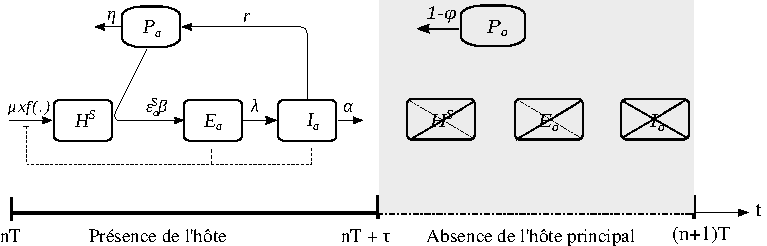
\includegraphics[width=1\linewidth]{semi_discret_NS.pdf}
		\caption[Diagramme compartimental de  la dynamique saisonnière de l'infection d'une plante sensible par des   
		nématodes avirulents.]{
		Ce diagramme compartimental  représente la dynamique saisonnière de l'infection pendant une année de longueur  
		$T$. La saisonnalité est caractérisée par  la succession de deux périodes : la saison de croissance, durant 
		laquelle la plante hôte est présente ($t \in (nT, nT + \tau])$, et la saison hivernale, qui représente 
		l'absence de la plante hôte et donc la phase de survie $(t \in (nT + \tau, (n + 1)T])$. Le compartiment $P_a$ 
		représente les densités de nématodes sous forme libre, $H^S$ les densités de racines racines  saines, $E_a$ 
		les densités de racines infectées de manière latente et $I_a$ les racines infectées quand les nématodes 
		produisent des œufs par reproduction clonale.  $\beta$ représente le taux de transmission; $r $ taux   
		reproduction du nématode ;  $\alpha$ et $\eta$ représentent le taux
		de mortalité des nématodes dans la plante et dans le sol respectivement.  
		Le trait plein de l’axe du temps représente les phénomènes continus (cycles d’infection sur des racines    
		sensibles par les nématodes avirulents). Le trait discontinu représente les phases de survie de l'agent 
		pathogène  (\textit{e.g.} la phase de survie hivernale) pendant l’intersaison (zone grise). Adapté de 
		\citet{Mailleret2012}.}
	\label{semi:discrete_nilusmas}
\end{figure}
	
	
\subsection{Introduction des génotypes virulents} \label{sec:introduction-virulents}
	
	Enfin, dans cette partie nous avons choisi de décrire le modèle complet qui  prend  en compte deux génotypes de plantes (résistant / sensible) et deux types de variants de nématodes (avirulent / virulent). Nous avons étendu le modèle~\eqref{eq:planteS-nemavir} pour introduire les nématodes virulents. L'indice $_v$   se réfère aux populations de nématodes virulents.  Le modèle étendu comporte trois nouvelles variables :  $P_v$ qui représente la densité de nématodes virulents sous forme libre dans le  sol;
$E_v$ qui représente les  densités de sites nourriciers infectés  de manière latente par les  virulents;  $I_v$ qui représente les  densités de sites nourriciers infectés par les virulents.   
	 
	Dans ce modèle, les populations de nématodes avirulentes $P_a$ et virulents $P_v$ durant la saison culturale sont en présence de  densités de racines saines $H^X$ d'une culture hôte  sensible ($X=S$)   ou résistante ($X=R$). À l'aide de deux sous modèles, nous avons choisir de décrire la modélisation de saisons de cultures,  soit avec des plantes sensibles ou résistantes.
	 

\subsubsection{Interaction d'une plante sensible -- nématodes avirulents et virulents}
	
	Nous représentons le modèle dans un diagramme de l'interaction entre une plante sensible et les populations de nématodes avirulents et virulents  par la \autoref{mod-sensible} :

\begin{figure}[H]
	\centering 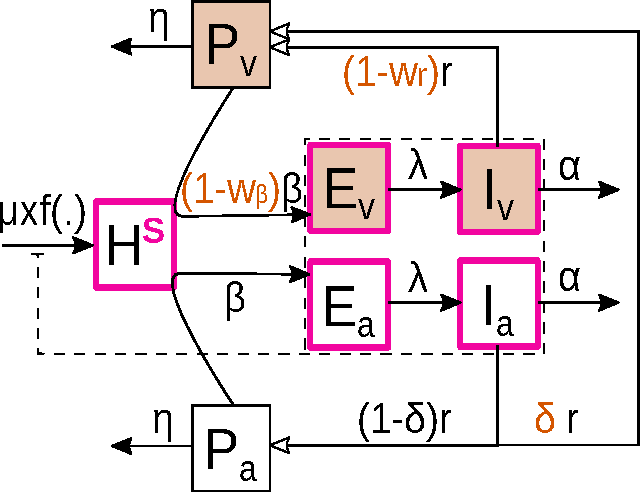
\includegraphics[width=0.5\linewidth]{mod_planteS.pdf}
		\caption[Modèle d'infection d'une plante sensible par des 
		nématodes avirulents et virulents]{
		Ce diagramme représente la dynamique d’infection sur une plante 
		saine $H^S$   par des nématodes virulents $P_v$   
	    	et avirulents $P_a$, avant de devenir infectée de manière 
	    	latente ($E_v$  et $E_a$) ensuite infectieuse ($I_v$  
		et $I_a$) quand les nématodes virulents et avirulents  pondent 
		par
		reproduction asexuée ou clonale. $\beta$ correspond au taux 
		d’infection entre les plantes et
		les nématodes ; $\lambda$ désigne le taux de passage du 
		compartiment $E$ à $I$ ; $r$ désigne le taux
		de reproduction des nématodes ; $\eta$ est le taux de mortalité 
		des nématodes dans le sol et
		$\alpha$ le taux de mortalité des nématodes dans la plante. Il 
		faut noter que les nématodes virulents se   
		développent  plus lentement que les avirulents parce qu'ils 
		souffrent de coûts de virulence, à deux niveaux : 
		une baisse sur l'infection $(w_\beta)$ 
		et une autre sur la  reproduction $(w_r)$. $\delta$ est la 
		fréquence d’évolution des descendants de nématodes avirulents à 
		virulents.}
		\label{mod-sensible}
\end{figure}
	
	Le système d'équation associé est le suivant :
		
\begin{equation}
	\left\{
		\begin{aligned}
		\dot{P_a} & =- \beta P_aH^S -\eta P_a + (1-\delta)r I_a,&\\
		\dot{P_v} & =-\beta P_vH^S -\eta P_v + \delta r I_a +(1-w_{r})r I_v,&\\
		\dot{H^S} &= \mu x f(H^S,E_a,E_v,I_v,I_a)-\epsilon_a^S  
		\beta P_a H^S-(1-w_{\beta}) \epsilon_v^S \beta P_v H^S,& \\
		\dot{E_a} &= \epsilon_a^S \beta P_a H^S  - \lambda E_a, &\\
		\dot{E_v} &=  (1-w_{\beta}) \epsilon_v^S \beta P_v H^S  - \lambda E_v, &\\
		\dot{I_a} & = \lambda E_a - \alpha I_a ,&\\
		\dot{I_v} & = \lambda E_v - \alpha I_v .&\\
		\end{aligned}
	\right.
	\label{eq:mod-sensible}
\end{equation}
avec $f(H^S,E_a,E_v,I_v,I_a)= e^{-k \pi}$ et $ \pi= \frac{E_a+E_v+I_v+I_a}{H^S+E_a+,E_v+I_v+I_a}$. 	
	
	 Par ce modèle nous pouvons modéliser les saisons de culture, de période $\tau$, de plantes sensibles
. Deux types de nématodes sont en compétition pour la plante saine $H^S$ : (i) les nématodes avirulents
$P_a$ peuvent infecter les plantes sensibles ($\epsilon^S_a =1$); (ii) 
les nématodes virulents $P_v$  sont capables d'infecter 
les plantes sensibles ($\epsilon^S_v =1$), mais ils se développent de manière moins efficace 
sur les plantes sensibles car l'acquisition de la virulence est associée
à des coûts de virulence. Les coûts de virulence sont susceptibles de se manifester à deux niveaux :  une baisse sur l'infectivité $(w_\beta)$ 
et une autre sur la  reproduction $(w_r)$ \citep{Jarquin-Barberena1991, Castagnone-Sereno2007, Meher2009,
 Djian-Caporalino2011}. $\delta$ est la fraction
d’apparition de descendants de nématodes avirulentes à virulents.
La densité initiale de la population totale de nématode $P_0$ est composée de nématodes
avirulents et virulents. En outre, nous avons supposé qu'une fraction $\delta$ des
descendants de nématodes avirulents sont virulents \citep{Castagnone-Sereno1994},
en raison de mutations et/ou de mécanismes épigénétiques. Selon les résultats de laboratoire
montrant que la virulence est un caractère 
stable chez le nématode \citep{Castagnone-Sereno1993},
nous avons également supposé que, une fois acquise, la virulence
ne pouvait pas être perdue par la lignée virulente.
	 
\subsubsection{Interaction plante résistante -- nématodes avirulents et virulents} \label{sec:model-resistance-precoce}
	
	Nous représentons le modèle dans un diagramme de l'interaction entre une plante sensible et les populations de nématodes avirulentes et virulents  par la \autoref{fig:resistance_tardive}a dans \Cref{annexeChap5}.
		
		\iffalse
\begin{figure}[H] 
	\centering 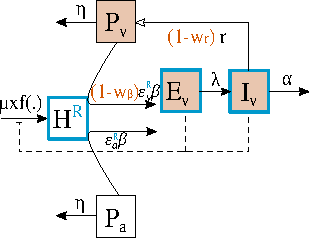
\includegraphics[width=0.5\linewidth]{mod_planteR.pdf}
		\caption[Modèle  de résistance précoce]{Ce diagramme représente la dynamique d’infection sur une plante saine $H^R$
		par des nématodes virulents $P_v$,   avant   
		de devenir infectée de manière latente $E_v$ ensuite infectieuse
		$I_v$ quand les nématodes virulents  pondent par
		reproduction asexuée ou clonale. Les nématodes avirulents
		$P_a$ sont incapables d'infecter et de se reproduire sur
		la plante résistante $(\epsilon_a^R=0)$. $\beta$ correspond au
		taux d’infection entre les plantes et
		les nématodes ; $\lambda$ désigne le taux de passage 
		du compartiment $E_v$ à $I_v$ ; $r$ désigne le taux
		de reproduction des nématodes ; $\eta$ est le taux de mortalité des nématodes dans le sol et
		$alpha$ le taux de mortalité des nématodes dans la plante.
		Il faut noter que les nématodes virulents souffrent de coûts de virulence, à deux niveaux : une baisse sur 
		l'infection $(w_\beta)$ 
		et une autre sur la  reproduction $(w_r)$. 
		}
		\label{fig:planteR-nemavir-vir}
\end{figure}
		\fi
	
Le système d'équation associé est le suivant :

\begin{equation}
	 \left\{
		\begin{aligned}
		\dot{P_a} & =- \beta P_aH^R -\eta P_a ,&\\
		\dot{P_v} & =-\beta P_vH^R -\eta P_v  +(1-w_{r})r I_v,&\\
		\dot{H^R} &= \mu x f(H^R,E_v,I_v) -(1-w_{\beta}) \epsilon_v^R \beta P_v H^R,& \\
		\dot{E_v} &=  (1-w_{\beta}) \epsilon_v^R \beta P_v H^R  - \lambda E_v, &\\
		\dot{I_v} & = \lambda E_v -\alpha I_v .&\\
		\end{aligned}
	\right.
\label{eq:ResistanceP-nemavir-nemvir}
\end{equation}
avec $f(H^R,E_v,I_v)= e^{-k \pi}$ et $ \pi= \frac{E_v+I_v }{H^R+E_v+I_v}$.
	
	Par ce modèle nous pouvons modéliser les saisons de culture de plantes résistantes. Ce modèle de résistance décrit une résistance précoce.
Ici, une fois qu'un nématode avirulent sous sa forme libre  pénètre dans la racine d'une plante résistante $H^R$ il est piégé au niveau du cortex  racinaire de la plante résistante ($\epsilon_a^R=0$). Ceci est dû à  une réaction d'hypersensibilité, c'est-à-dire  une mort rapide et localisée des cellules végétales autour du
nématode à cause de l’expression d’un gène de résistance, empêchant le développement et la multiplication du nématode.  Contrairement à l'interaction avec une plante sensible, les nématodes avirulents  $P_a$  sont incapables d'infecter les plantes résistantes et de se développer. Ceci  explique pourquoi les variables $I_a$ et $E_a$ sont absentes. Les nématodes virulents $P_v$ sont capables d'infecter les plantes résistantes et sensibles ($\epsilon_v^R$= 1), mais l'acquisition de la virulence  est également associée aux coûts de virulence. Les coûts de virulence sont aussi susceptibles de se manifester aux niveaux de l'infectivité $(w_\beta)$  et de la  reproduction $(w_r)$. Dans une interaction impliquant un gène R,  il peut exister ce que l'on appelle  un coût de fitness additionnel ou \og effet résiduel \fg{} de la plante résistante. Dans ce cas, on peut observer une différence de niveau entre le potentiel reproducteur des virulents se développant sur une plante sensible et sur une plante  résistante qui serait liée à un manque d’efficacité de la résistance.  Une analyse  statistique plus approfondie, nous a montré qu’il n’y a pas d’effet résiduel de la résistance portant  le gène \textit{Mi-1} \citep{Castagnone-Sereno2007}. Les coûts de virulence sont donc identiques sur plante sensible et résistante.
Dans ce modèle, la fraction $\delta$ des descendants de nématodes avirulents en virulents est absente car il n'y a pas de nématodes avirulents qui peuvent se développer sur une plante résistante.    
	
	Le modèle saisonnier complet est donc l'ensemble de ces deux sous modèles \eqref{eq:mod-sensible} et   \eqref{eq:ResistanceP-nemavir-nemvir} associés à une séquence de rotation entre plantes sensibles et résistantes.
Les conditions initiales du modèle multi-saisonnier complet ont été fixées à $H^X (0) = H_0$, les
biomasses initiales des racines des hôtes nouvellement plantés, $P_a = (1-p_v)P_0$ et $P_v = p_v P_0$ , où
$P_0$ se réfère à la densité initiale des nématodes dans le sol et $p_v$ à la proportion initiale de
des nématodes virulents dans le sol. Les valeurs initiales de $I_a$ , $E_a$ , $I_v$ et $E_v$ ont été fixées à 0 parce que les plantes étaient supposées être saines au moment où elles étaient plantées.
À la fin de chaque saison de culture, les plantes sont arrachées. Au début de la prochaine
saison de culture, les racines saines et infectées sont ainsi ramenées à leurs valeurs initiales, $H_0$ et
0, respectivement. Les densités de nématodes $P_a$ et $P_v$ sont fixées à leur valeur à la fin de la
saison de culture précédente, multipliée par une probabilité de survie $\varphi$. On suppose que l'intersaison n'a pas d'effet différentiel selon que les nématodes soient virulents ou non (pas de sélection à l'intersaison).
Cette partie du modèle est calculée par une équation discrète de la manière suivante :
	 
	
	\begin{equation}
		\left\{
		 \begin{aligned}
		    P_a ((n+1)T) &= \varphi P_a(nT + \tau),\\
		    P_v ((n+1)T) &= \varphi P_v(nT + \tau).
		 \end{aligned}
		\right.
		\label{eq:intersaison-nemavir-nemvir}
	\end{equation}

	
	
	Le modèle complet de la plante L'interaction des nématodes sur plusieurs saisons de culture est donc un modèle hybride, avec une
partie continue pour décrire la dynamique de l'infection par les nématodes pendant une saison de culture
de longueur $\tau$ , et une partie discrète pour décrire la survie des nématodes entre les saisons (\autoref{semi:discrete_complet_nilusmas}).
	
	
	
	\begin{figure}	
		\centering 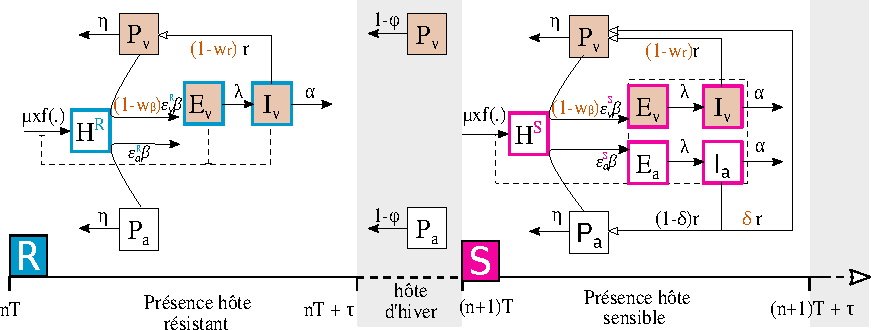
\includegraphics[width=1\linewidth]{semi_discret_comp_NS.pdf}
		\caption[Diagramme compartimental de  la dynamique saisonnière de l'infection d'une plante sensible ($X = S$) 
		ou résistante ($ X=R $) par des nématodes avirulents et virulents.]{
		Diagramme compartimental représentant le modèle d'interaction plante-nématode
		pour deux saisons de culture successives de plantes résistantes ($X = R$) et sensibles ($X = S$). La 
		saisonnalité est caractérisée par  la succession de deux périodes : la saison de croissance, durant laquelle la 
		plante hôte est présente ($t \in (nT, nT + \tau])$, et la saison hivernale, qui représente l'absence de la 
		plante hôte et donc la phase de survie $(t \in (nT + \tau, (n + 1)T])$. Les racines saines des plantes ($H^X$) 
		sont infectées par des nématodes virulents (indice $_v$) et avirulents (indice $_a$) dans le sol ($P$), avant 
		de devenir infectées de manière latente ($E = E_a + E_v $), puis infectieux ($I = I_a + I_v$) .  $\beta$ 
		représente le taux de  transmission; $r $ taux   reproduction du nématode ;  $\alpha$ et $\eta$ représentent le 
		taux de mortalité des nématodes dans la plante et dans le sol respectivement.  
		Le trait plein de l’axe du temps représente les phénomènes continus (cycles d’infection sur des racines 
		sensibles ou résistantes par les nématodes avirulents et virulents). Le trait discontinu représente les phases 
		de survie des nématodes avirulents et virulents (\textit{e.g.} la phase de survie hivernale) pendant 
		l’intersaison en condition de cultures (zone grise). Adapté de \citet{Mailleret2012}.}	
		\label{semi:discrete_complet_nilusmas}
	\end{figure}

	
	
	 Dans l'esprit de~\ref{sec:ext}~\autoref{sec:resist-virul}, nous étudierons des stratégies de déploiement de la résistance pour une gestion efficace et durable d'agents pathogènes de plantes. Nous nous concentrons particulièrement sur les rotations car ce sont celles qui ont montré leur efficacité sur le contrôle des nématodes à galles.  Ce nouveau cadre de modélisation a  permis en premier lieu la recherche de stratégies optimales de déploiement de différents  gènes de résistance, et l'évaluation de la robustesse de ces stratégies. C'est l'objet du chapitre suivant qui est présenté sous forme d'article.
	
	
	
	
	
	
	%\bibliographystyle{newphy}
	%\bibliography{mybiblio}
